\documentclass[11pt, a4paper, oneside]{report}

% ==================== PACKAGES ====================
\usepackage[utf8]{inputenc}
\usepackage[T1]{fontenc}
\usepackage[a4paper, margin=2.5cm, top=3cm, bottom=3cm]{geometry}
\usepackage{lmodern}

% Mathematics
\usepackage{amsmath, amssymb, amsfonts}

% Colors
\usepackage{xcolor}
\definecolor{primary}{RGB}{14, 116, 144}      % Cyan/Teal
\definecolor{secondary}{RGB}{30, 41, 59}     % Slate Dark
\definecolor{accent}{RGB}{225, 29, 72}       % Rose
\definecolor{amber}{RGB}{245, 158, 11}
\definecolor{emerald}{RGB}{16, 185, 129}
\definecolor{indigo}{RGB}{99, 102, 241}
\definecolor{slate}{RGB}{100, 116, 139}
\definecolor{codegreen}{RGB}{46, 125, 50}
\definecolor{codeblue}{RGB}{21, 101, 192}
\definecolor{codegray}{RGB}{120, 144, 156}
\definecolor{codebg}{RGB}{248, 250, 252}

% TikZ & Schematics
\usepackage{tikz}
\usetikzlibrary{
    shapes.geometric, 
    arrows.meta, 
    positioning, 
    calc, 
    fit, 
    backgrounds, 
    decorations.pathreplacing
}

% Tables
\usepackage{booktabs}
\usepackage{tabularx}
\usepackage{multirow}
\usepackage{array}

% Code Listings
\usepackage{listings}
\lstdefinestyle{vhdlstyle}{
    backgroundcolor=\color{codebg},
    commentstyle=\color{codegray}\itshape,
    keywordstyle=\color{codeblue}\bfseries,
    numberstyle=\tiny\color{codegray},
    stringstyle=\color{codegreen},
    basicstyle=\ttfamily\footnotesize,
    breakatwhitespace=false,
    breaklines=true,
    captionpos=b,
    keepspaces=true,
    numbers=left,
    numbersep=7pt,
    showspaces=false,
    showstringspaces=false,
    showtabs=false,
    tabsize=2,
    frame=single,
    rulecolor=\color{black!20}
}
\lstdefinestyle{cstyle}{
    backgroundcolor=\color{codebg},
    commentstyle=\color{codegray}\itshape,
    keywordstyle=\color{accent}\bfseries,
    numberstyle=\tiny\color{codegray},
    stringstyle=\color{primary},
    basicstyle=\ttfamily\footnotesize,
    breakatwhitespace=false,
    breaklines=true,
    captionpos=b,
    keepspaces=true,
    numbers=left,
    numbersep=7pt,
    showspaces=false,
    showstringspaces=false,
    showtabs=false,
    tabsize=4,
    frame=single,
    rulecolor=\color{black!20}
}
\lstset{style=vhdlstyle}

% Headers & Footers
\usepackage{fancyhdr}
\pagestyle{fancy}
\fancyhf{}
\fancyhead[L]{\small\color{secondary}\textbf{spGPU}: 2D/2.5D Multicore FPGA GPU}
\fancyhead[R]{\small\color{secondary}\nouppercase{\leftmark}}
\fancyfoot[C]{\thepage}
\renewcommand{\headrulewidth}{0.5pt}
\renewcommand{\footrulewidth}{0pt}

% Hyperref
\usepackage{hyperref}
\hypersetup{
    colorlinks=true,
    linkcolor=primary,
    citecolor=emerald,
    urlcolor=accent,
    pdfauthor={Luca Filogna and Valerio Cilento},
    pdftitle={spGPU: Complete Architecture and System Documentation},
    pdfsubject={Hardware/Software Co-Design of a 2D/2.5D Multicore GPU on FPGA}
}

% Title formatting
\usepackage{titlesec}
\titleformat{\chapter}[display]
  {\normalfont\huge\bfseries\color{secondary}}
  {\filleft\Huge\color{primary}\chaptertitlename\ \thechapter}
  {4ex}
  {\titlerule[1.5pt]\vspace{2ex}\filright}
  [\vspace{2ex}\titlerule]

% ==================== DOCUMENT METADATA ====================
\title{
    \vspace{-2.0cm}
    \Huge\textbf{\color{primary}spGPU: Architecture and System Specification}\\[0.4cm]
    \LARGE\textbf{Design, Implementation, and Evaluation of a 2D/2.5D Multicore Tiled Graphics Processing Unit on FPGA SoC}\\[0.8cm]
    \large Digital Signal Processing (DSP) Course Project\\
    Sapienza University of Rome
}

\author{
    \textbf{Luca Filogna} \quad \& \quad \textbf{Valerio Cilento}\\[0.2cm]
    \textit{Faculty of Information Engineering, Computer Science and Statistics}\\
    \textit{Department of Information Engineering, Electronics and Telecommunications (DIET)}\\
    \textit{Sapienza University of Rome, Italy}
}

\date{\textbf{Academic Year 2025--2026}\\[0.4cm] \small Revision 2.1 -- Full System Documentation}

% ==================== DOCUMENT BODY ====================
\begin{document}

\maketitle

\begin{abstract}
This report provides a comprehensive architectural and engineering specification of \textbf{spGPU}, a custom, high-performance 2D/2.5D multicore Graphics Processing Unit implemented on a Xilinx Zynq-7000 All-Programmable System-on-Chip (SoC) hosted on the Digilent PYNQ-Z1 development board. 

spGPU adopts a spatially partitioned, tile-based architecture comprising ten independent compute cores (\texttt{spCORE}) executing in parallel at $100.0\,\text{MHz}$. Each core is tightly coupled to a dedicated on-chip True Dual-Port Block RAM tile ($320 \times 24$ pixels), providing a total rendering resolution of $320 \times 240$ with 15-bit RGB555 color depth. Dedicated integer hardware rasterization engines accelerate geometric primitives, including Bresenham lines, midpoint circles, solid disc scanlines, and edge-equation triangle fills.

An integrated 4-bit depth buffer (Z-buffer) is implemented in every tile memory, executing single-cycle depth comparisons to resolve occlusion and 2.5D layering autonomously. A dynamic instruction scheduler calculates primitive bounding boxes in combinational logic, streaming 64-bit spISA commands exclusively to the overlapping tile FIFOs to maximize compute efficiency. The video subsystem provides $2\times$ hardware nearest-neighbor upscaling, TMDS 8b/10b encoding, and 5:1 DDR serialization at $125.0\,\text{MHz}$ via \texttt{OSERDESE2} primitives, driving an HDMI display at $640 \times 480$ @ $60\,\text{Hz}$ with zero tearing through VSYNC-locked ping-pong double buffering. 

A dual-interrupt synchronization architecture connects the GPU to an ARM Cortex-A9 host running a bare-metal Newtonian physics engine, demonstrating rock-solid 60 FPS performance verified through desktop visual co-simulation and hardware synthesis.
\end{abstract}

\tableofcontents
\listoffigures
\listoftables

% ==================== CHAPTERS ====================
\chapter{Introduction and Project Overview}
\label{chap:introduction}

\section{Academic Context and Project Scope}
The \textbf{spGPU} (\textit{Sapienza Graphics Processing Unit}) project was conceived, designed, and implemented as an advanced digital design and hardware acceleration project for the \textit{Digital Signal Processing (DSP)} course at \textbf{Sapienza University of Rome}, authored by \textbf{Luca Filogna} and \textbf{Valerio Cilento}.

The primary objective of the project is the full-stack design, algorithmic prototyping, Register-Transfer Level (RTL) implementation in VHDL, software simulation, and physical FPGA synthesis of a custom \textbf{2D/2.5D Multicore Graphics Processing Unit}. Rather than relying on commercial graphics IP cores or software-driven framebuffers, spGPU represents an entirely custom hardware architecture featuring parallel compute pipelines, distributed on-chip video memory, hardware rasterizers, an integrated depth buffer (Z-buffer), and a direct High-Definition Multimedia Interface (HDMI) physical transmitter.

\section{Target Hardware Platform}
The complete system is synthesized and validated on the \textbf{Digilent PYNQ-Z1} development board, built around the \textbf{Xilinx Zynq-7000 All-Programmable SoC (\texttt{XC7Z020-1CLG400C})}. The architecture takes full advantage of the heterogeneous SoC paradigm:
\begin{itemize}
    \item \textbf{Processing System (PS)}: Hosts a Dual-Core ARM Cortex-A9 MPCore microprocessor operating up to $667\,\text{MHz}$, responsible for running the application game loop, rigid-body physics simulation, collision detection, and issuing drawing commands.
    \item \textbf{Programmable Logic (PL)}: Implements the spGPU multicore processor, the instruction dispatcher, the distributed dual-port Block RAM framebuffers, the hardware Z-buffer, the hardware performance monitor, and the HDMI physical layer.
    \item \textbf{On-Chip Interconnect}: High-throughput AXI4 interfaces and an AXI Direct Memory Access (DMA) engine in Simple Mode that streams graphics instructions directly from the ARM memory space into the GPU instruction scheduler.
\end{itemize}

\section{Key Architectural Specifications}
Table~\ref{tab:system_specs} summarizes the fundamental architectural parameters and performance metrics of the spGPU system.

\begin{table}[htbp]
\centering
\caption{spGPU Hardware Architectural Specifications}
\label{tab:system_specs}
\begin{tabular}{@{}ll@{}}
\toprule
\textbf{Parameter} & \textbf{Specification / Value} \\ \midrule
Target Device & Xilinx Zynq-7000 SoC (\texttt{xc7z020clg400-1}) \\
Development Board & Digilent PYNQ-Z1 \\
Synthesis Toolflow & AMD Xilinx Vivado 2023.1 \\
Host Processor (PS) & Dual-Core ARM Cortex-A9 (Bare-Metal C) \\
GPU Clock Domain & $100.0\,\text{MHz}$ (Core compute, memory write, scheduler) \\
Pixel Clock Domain & $25.0\,\text{MHz}$ (Display scanning, VGA timing generator) \\
Serial Clock Domain & $125.0\,\text{MHz}$ ($5\times$ pixel clock, TMDS 5:1 DDR serialization) \\
Logical Rendering Resolution & $320 \times 240$ pixels \\
Physical HDMI Output & $640 \times 480$ @ $60\,\text{Hz}$ (Standard 480p VGA timing) \\
Hardware Spatial Upscaler & $2\times$ Horizontal \& $2\times$ Vertical Nearest-Neighbor \\
Color Representation & 15-bit RGB555 ($32{,}768$ colors), expanded to 24-bit RGB888 \\
Depth Buffer (Z-Buffer) & Integrated 4-bit per pixel (16 discrete depth layers) \\
Spatial Parallelism & 10 Independent Compute Cores (\texttt{spCORE}) \\
Tiling Geometry & 10 Horizontal Tiles of $320 \times 24$ pixels each \\
On-Chip VRAM Structure & 10 Distributed True Dual-Port Block RAM tiles \\
Buffering Scheme & Double-Buffering (Ping-Pong VRAM) with VSYNC-lock \\
Background Auto-Clear & Hardware zero-overhead back-buffer clearing upon swap \\
Communication Protocol & AXI DMA (Memory-Mapped to Stream) + 64-bit spISA \\
Hardware Telemetry & Integrated 100 MHz FPS counter with dual GIC interrupts \\ \bottomrule
\end{tabular}
\end{table}

\section{Design Methodology and Toolflow}
The engineering lifecycle followed for spGPU adopted a rigorous, verification-driven methodology:
\begin{enumerate}
    \item \textbf{Software Prototyping \& Golden Models}: High-level C/C++ algorithms were formulated for all primitive rasterization techniques (Bresenham lines, midpoint circles, scanline spans, and edge-equation half-space triangle filling) and OpenCV-based nearest-neighbor scaling.
    \item \textbf{Visual RTL Co-Simulation}: A desktop graphical simulator was constructed using the \textit{Raylib} library, capable of consuming pixel dump files generated during VHDL testbench simulations and rendering the exact visual frame to verify circuit correctness before FPGA implementation.
    \item \textbf{RTL Synthesis and Place-and-Route}: Synthesized using AMD Vivado 2023.1, enforcing multi-clock domain constraints (100 MHz core clock, 25 MHz pixel clock, 125 MHz serial clock) and optimizing logic placement across the 28nm Artix-7 fabric.
    \item \textbf{Bare-Metal Integration}: Construction of memory-mapped peripheral drivers, interrupt service routines (ISRs) via the ARM Generic Interrupt Controller (GIC), and deployment via bootable SD card images (\texttt{BOOT.bin}).
\end{enumerate}

\chapter{System-on-Chip (SoC) Architecture and Interconnect}
\label{chap:soc_architecture}

\section{System Partitioning: Processing System vs. Programmable Logic}
The spGPU architecture adopts a hardware/software co-design strategy that leverages the Xilinx Zynq-7000 All-Programmable System-on-Chip (SoC). The system is physically partitioned into two tightly coupled domains:
\begin{enumerate}
    \item \textbf{Processing System (PS)}: Hosts the dual-core ARM Cortex-A9 processor running bare-metal C firmware. The CPU executes high-level tasks that require complex branching, floating-point calculations, and dynamic state evaluation, including rigid-body physics, ball-to-ball and boundary elastic collision resolution, and frame timing orchestration.
    \item \textbf{Programmable Logic (PL)}: Implements the spGPU coprocessor, containing the instruction dispatching unit, the parallel compute cores, the distributed tile memories, the performance analyzer, and the physical HDMI output engine.
\end{enumerate}

Figure~\ref{fig:soc_overview} illustrates the global block diagram of the SoC architecture, highlighting the interconnect interfaces, clock domains, and interrupt lines connecting the ARM processor with the FPGA logic.

\begin{figure}[htbp]
\centering
\resizebox{0.95\textwidth}{!}{
    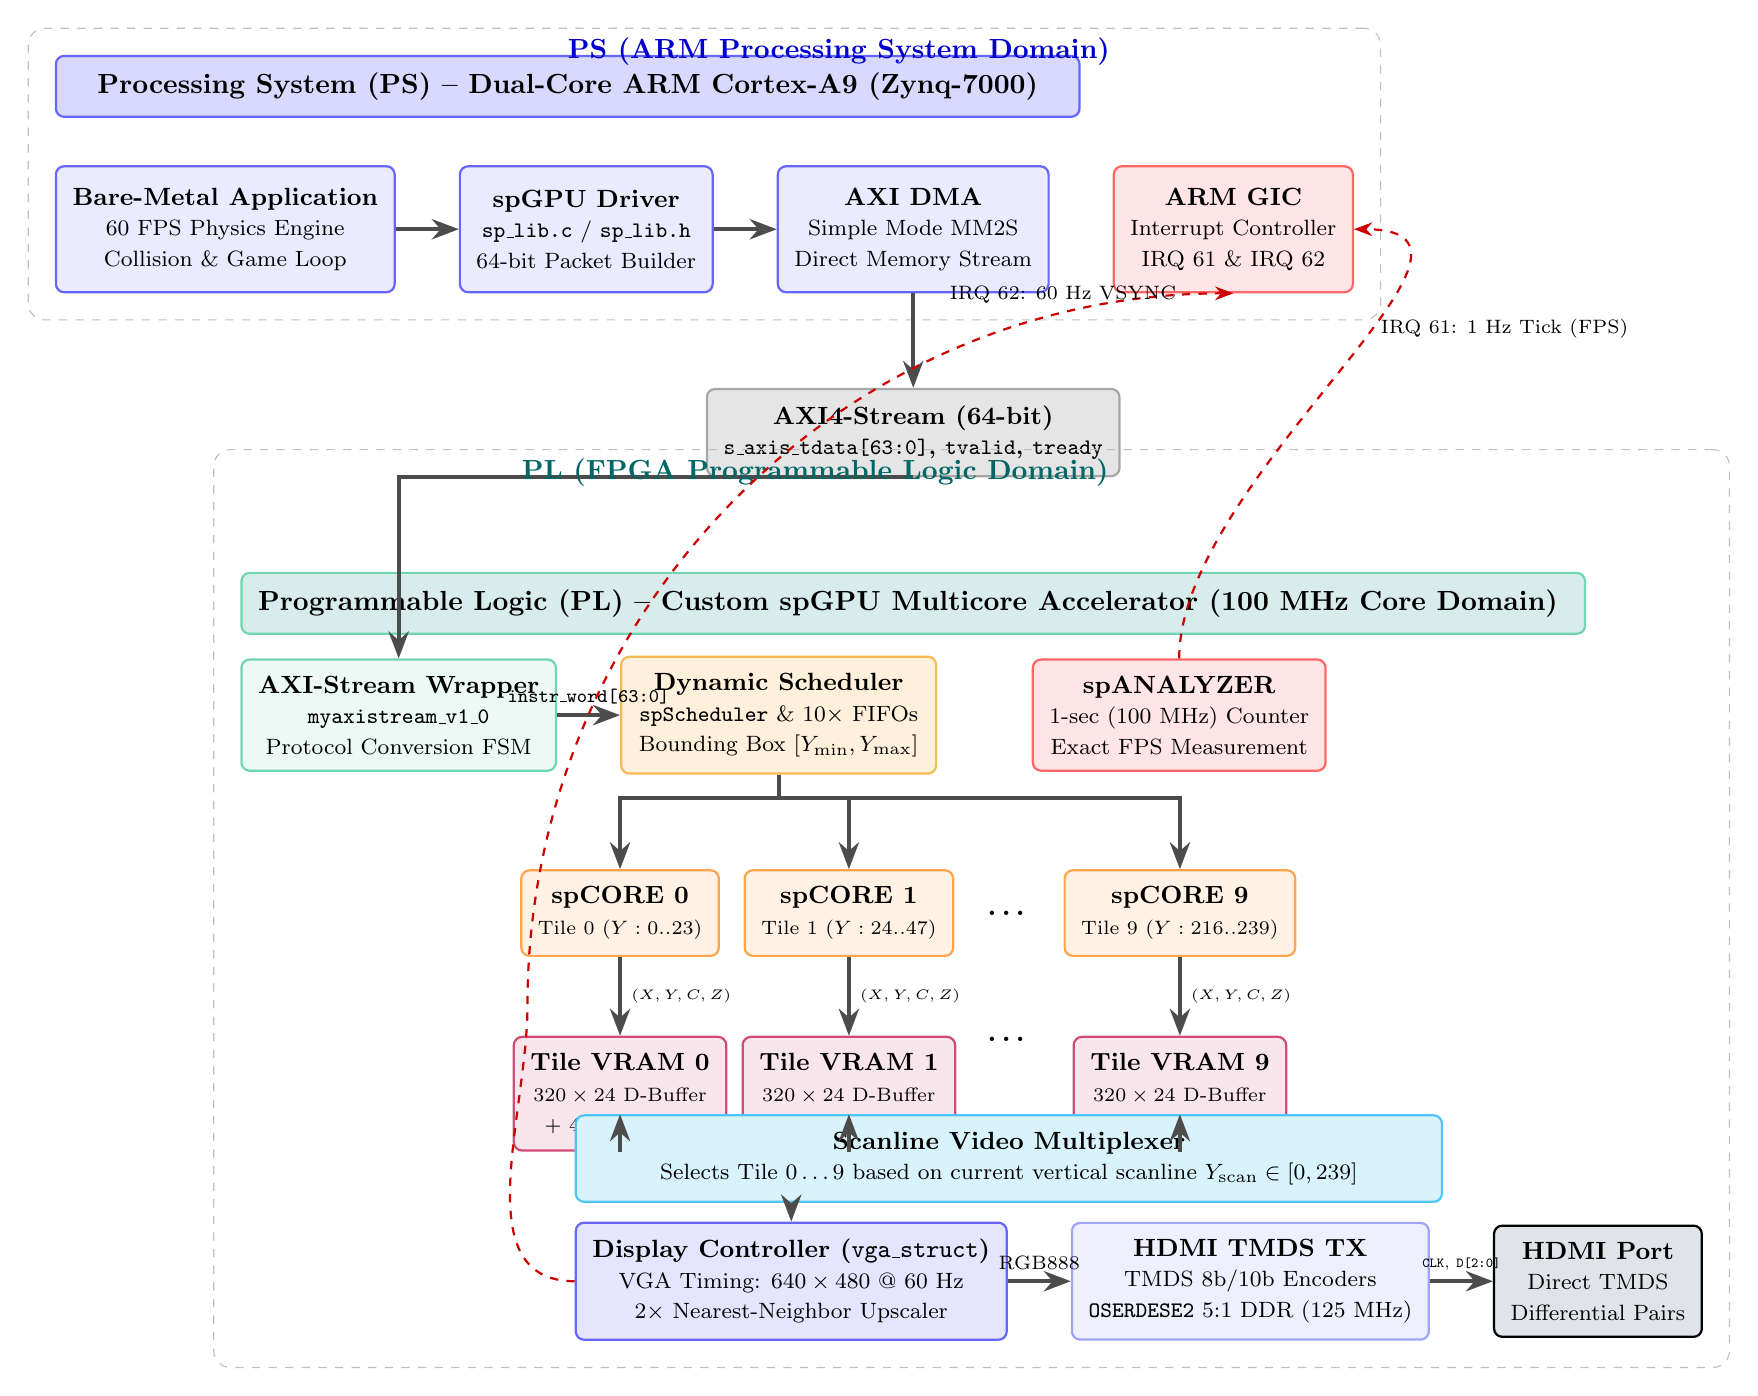
\begin{tikzpicture}[
    >=Stealth,
    node distance=1.2cm and 1.5cm,
    every text node part/.style={align=center},
    box/.style={draw=black!80, thick, rounded corners=3pt, fill=white, inner sep=6pt, font=\small},
    psbox/.style={box, fill=blue!8, draw=blue!60},
    plbox/.style={box, fill=emerald!8, draw=emerald!60},
    corebox/.style={box, fill=orange!10, draw=orange!70, minimum width=2.2cm, minimum height=0.9cm},
    tilebox/.style={box, fill=purple!10, draw=purple!70, minimum width=2.2cm, minimum height=0.9cm},
    bus/.style={draw=black!70, line width=1.5pt, ->},
    sig/.style={draw=blue!70!black, thick, ->},
    intsig/.style={draw=red!80!black, thick, dashed, ->},
    subframe/.style={draw=gray!50, dashed, rounded corners=6pt, inner sep=10pt}
]

% ==================== PROCESSING SYSTEM (PS) ====================
\begin{scope}[local bounding box=ps_box]
    \node[psbox, font=\bfseries\normalsize, fill=blue!15, minimum width=13cm] (ps_title) {Processing System (PS) -- Dual-Core ARM Cortex-A9 (Zynq-7000)};
    
    \node[psbox, below=0.6cm of ps_title.south west, anchor=north west, minimum width=3.2cm, minimum height=1.6cm] (arm_app) {
        \textbf{Bare-Metal Application}\\
        \footnotesize 60 FPS Physics Engine\\
        \footnotesize Collision \& Game Loop
    };
    
    \node[psbox, right=0.8cm of arm_app, minimum width=3.0cm, minimum height=1.6cm] (arm_lib) {
        \textbf{spGPU Driver}\\
        \footnotesize\texttt{sp\_lib.c} / \texttt{sp\_lib.h}\\
        \footnotesize 64-bit Packet Builder
    };

    \node[psbox, right=0.8cm of arm_lib, minimum width=2.4cm, minimum height=1.6cm] (axi_dma) {
        \textbf{AXI DMA}\\
        \footnotesize Simple Mode MM2S\\
        \footnotesize Direct Memory Stream
    };

    \node[psbox, fill=red!10, draw=red!60, right=0.8cm of axi_dma, minimum width=2.2cm, minimum height=1.6cm] (gic) {
        \textbf{ARM GIC}\\
        \footnotesize Interrupt Controller\\
        \footnotesize IRQ 61 \& IRQ 62
    };

    \draw[bus] (arm_app) -- (arm_lib);
    \draw[bus] (arm_lib) -- (axi_dma);
\end{scope}
\node[subframe, fit=(ps_box), label={[anchor=north west, font=\bfseries\color{blue!80!black}]above left:PS (ARM Processing System Domain)}] {};

% ==================== INTERCONNECT ====================
\node[box, fill=gray!20, draw=gray!70, below=1.2cm of axi_dma, minimum width=3.8cm, font=\small\bfseries] (axi_stream) {
    AXI4-Stream (64-bit)\\
    \footnotesize\texttt{s\_axis\_tdata[63:0]}, \texttt{tvalid}, \texttt{tready}
};
\draw[bus] (axi_dma) -- (axi_stream);

% ==================== PROGRAMMABLE LOGIC (PL) ====================
\begin{scope}[local bounding box=pl_box]
    \node[plbox, fill=teal!15, font=\bfseries\normalsize, below=1.2cm of axi_stream, minimum width=15.5cm] (pl_title) {
        Programmable Logic (PL) -- Custom spGPU Multicore Accelerator (100 MHz Core Domain)
    };

    \node[plbox, below=0.7cm of pl_title.west, anchor=north west, minimum width=3.4cm, minimum height=1.2cm] (axi_wrap) {
        \textbf{AXI-Stream Wrapper}\\
        \footnotesize\texttt{myaxistream\_v1\_0}\\
        \footnotesize Protocol Conversion FSM
    };
    \draw[bus] (axi_stream.south) -| (axi_wrap.north);

    \node[plbox, fill=amber!15, draw=amber!70, right=0.8cm of axi_wrap, minimum width=4.0cm, minimum height=1.2cm] (sched) {
        \textbf{Dynamic Scheduler}\\
        \footnotesize\texttt{spScheduler} \& 10$\times$ FIFOs\\
        \footnotesize Bounding Box $[Y_{\min}, Y_{\max}]$
    };
    \draw[bus] (axi_wrap) -- node[above, font=\scriptsize] {\texttt{instr\_word[63:0]}} (sched);

    \node[plbox, fill=red!10, draw=red!60, right=1.2cm of sched, minimum width=3.2cm, minimum height=1.2cm] (analyzer) {
        \textbf{spANALYZER}\\
        \footnotesize 1-sec (100 MHz) Counter\\
        \footnotesize Exact FPS Measurement
    };

    % Core Array
    \node[corebox, below=1.2cm of sched.south west, anchor=north] (c0) {\textbf{spCORE 0}\\ \scriptsize Tile 0 ($Y: 0..23$)};
    \node[corebox, right=0.3cm of c0] (c1) {\textbf{spCORE 1}\\ \scriptsize Tile 1 ($Y: 24..47$)};
    \node[font=\bfseries, right=0.3cm of c1] (cdots) {\dots};
    \node[corebox, right=0.3cm of cdots] (c9) {\textbf{spCORE 9}\\ \scriptsize Tile 9 ($Y: 216..239$)};

    % Tile BRAM Array
    \node[tilebox, below=1.0cm of c0] (t0) {\textbf{Tile VRAM 0}\\ \scriptsize $320\times 24$ D-Buffer\\ \scriptsize + 4-bit Z-RAM};
    \node[tilebox, below=1.0cm of c1] (t1) {\textbf{Tile VRAM 1}\\ \scriptsize $320\times 24$ D-Buffer\\ \scriptsize + 4-bit Z-RAM};
    \node[font=\bfseries, below=1.3cm of cdots] (tdots) {\dots};
    \node[tilebox, below=1.0cm of c9] (t9) {\textbf{Tile VRAM 9}\\ \scriptsize $320\times 24$ D-Buffer\\ \scriptsize + 4-bit Z-RAM};

    \draw[bus] (sched.south) -- ++(0,-0.3) -| (c0.north);
    \draw[bus] (sched.south) -- ++(0,-0.3) -| (c1.north);
    \draw[bus] (sched.south) -- ++(0,-0.3) -| (c9.north);

    \draw[bus] (c0) -- node[right, font=\tiny] {$(X,Y,C,Z)$} (t0);
    \draw[bus] (c1) -- node[right, font=\tiny] {$(X,Y,C,Z)$} (t1);
    \draw[bus] (c9) -- node[right, font=\tiny] {$(X,Y,C,Z)$} (t9);

    % Scanline Multiplexer
    \node[box, fill=cyan!15, draw=cyan!70, below=0.8cm of tdots, minimum width=11cm, minimum height=0.9cm] (mux) {
        \textbf{Scanline Video Multiplexer}\\
        \footnotesize Selects Tile $0 \dots 9$ based on current vertical scanline $Y_{\text{scan}} \in [0, 239]$
    };
    \draw[bus] (t0.south) -- (t0.south |- mux.north);
    \draw[bus] (t1.south) -- (t1.south |- mux.north);
    \draw[bus] (t9.south) -- (t9.south |- mux.north);

    % Display Controller
    \node[box, fill=blue!10, draw=blue!60, below=0.8cm of mux.west, anchor=north west, minimum width=4.5cm] (vga) {
        \textbf{Display Controller (\texttt{vga\_struct})}\\
        \footnotesize VGA Timing: $640\times 480$ @ 60 Hz\\
        \footnotesize 2$\times$ Nearest-Neighbor Upscaler
    };
    \draw[bus] (mux.south -| vga.north) -- (vga.north);

    % TMDS & Serializer
    \node[box, fill=indigo!10, draw=indigo!60, right=0.8cm of vga, minimum width=3.8cm] (tmds) {
        \textbf{HDMI TMDS TX}\\
        \footnotesize TMDS 8b/10b Encoders\\
        \footnotesize\texttt{OSERDESE2} 5:1 DDR (125 MHz)
    };
    \draw[bus] (vga) -- node[above, font=\scriptsize] {RGB888} (tmds);

    \node[box, fill=slate!20, draw=black, right=0.8cm of tmds, minimum width=2.4cm] (hdmi_port) {
        \textbf{HDMI Port}\\
        \footnotesize Direct TMDS\\
        \footnotesize Differential Pairs
    };
    \draw[bus] (tmds) -- node[above, font=\tiny] {\texttt{CLK}, \texttt{D[2:0]}} (hdmi_port);

\end{scope}
\node[subframe, fit=(pl_box), label={[anchor=north west, font=\bfseries\color{teal!80!black}]above left:PL (FPGA Programmable Logic Domain)}] {};

% ==================== INTERRUPT CONNECTIONS ====================
\draw[intsig] (analyzer.north) to[out=90, in=0] node[pos=0.6, right, font=\scriptsize] {IRQ 61: 1 Hz Tick (FPS)} (gic.east);
\draw[intsig] (vga.west) to[out=180, in=-90] ++(-0.6, 3.5) to[out=90, in=180] node[pos=0.85, above, font=\scriptsize] {IRQ 62: 60 Hz VSYNC} (gic.south);

\end{tikzpicture}

}
\caption{spGPU System-on-Chip (SoC) Top-Level Architecture and Interconnect.}
\label{fig:soc_overview}
\end{figure}

\section{AXI DMA Communication Subsystem}
To offload graphics commands without burdening the CPU with per-pixel or per-word Programmed I/O (PIO) transactions, communication from the PS to the PL is mediated by the \textbf{Xilinx AXI Direct Memory Access (AXI DMA)} core configured in \textit{Simple Direct Register Mode} for Memory-Mapped to Stream (MM2S) transfers:
\begin{itemize}
    \item \textbf{High-Speed Memory Read}: The DMA controller accesses DDR memory over the 32-bit AXI High-Performance (HP) slave port on the PS.
    \item \textbf{Stream Conversion}: Instructions formatted into contiguous memory buffers are streamed over a 64-bit AXI4-Stream master interface (\texttt{M\_AXIS\_MM2S}).
    \item \textbf{Low Software Overhead}: The CPU merely writes the source address (\texttt{MM2S\_SA}) and transfer byte length (\texttt{MM2S\_LENGTH}) to the DMA memory-mapped control registers, allowing the hardware engine to burst instructions autonomously.
\end{itemize}

\section{AXI4-Stream Custom Peripheral (\texttt{myaxistream\_1\_0})}
The raw AXI4-Stream interface from the DMA engine is received on the FPGA by a custom conversion peripheral, \texttt{myaxistream\_1\_0} (detailed in \texttt{myaxistream\_v1\_0\_S\_AXIS.vhd}). This module serves as the primary gateway and protocol adapter between the Xilinx AXI bus and the internal scheduler of spGPU.

\subsection{State Machine and Handshaking}
The stream interface operates under a three-state Finite State Machine (FSM):
\begin{enumerate}
    \item \texttt{WAIT\_S}: The receiver remains in idle until the GPU scheduler asserts \texttt{ready\_enb} (indicating that the core FIFOs are ready to absorb a new command). Upon detecting a rising edge on \texttt{ready\_enb}, the FSM transitions to \texttt{TX1\_S}.
    \item \texttt{TX1\_S}: The core asserts \texttt{S\_AXIS\_TREADY <= '1'}, signalling to the DMA master that it is prepared to accept data. When \texttt{S\_AXIS\_TVALID} is sampled high, the FSM advances to \texttt{TX2\_S}.
    \item \texttt{TX2\_S}: The 64-bit data bus \texttt{S\_AXIS\_TDATA} is latched into \texttt{instr\_word}, \texttt{instr\_valid} is pulsed high for one cycle, \texttt{S\_AXIS\_TREADY} is deasserted, and the FSM returns to \texttt{WAIT\_S}.
\end{enumerate}

Listing~\ref{lst:axis_fsm} shows the core VHDL FSM implementation of this handshake protocol.

\begin{lstlisting}[language=VHDL, caption={AXI4-Stream Handshake and State Machine in \texttt{myaxistream\_v1\_0\_S\_AXIS.vhd}.}, label={lst:axis_fsm}]
process(all) 
begin
    if S_AXIS_ARESETN = '0' then
        next_state_t <= WAIT_S;
    else 
        case state_t is
            when WAIT_S => 
                if fsm_start_edge = '1' then
                    next_state_t <= TX1_S;
                else 
                    next_state_t <= WAIT_S;
                end if;
            when TX1_S =>
                if S_AXIS_TVALID = '1' then
                    next_state_t <= TX2_S;
                else 
                    next_state_t <= TX1_S;
                end if;
            when TX2_S =>
                next_state_t <= WAIT_S;
            when others => 
                next_state_t <= WAIT_S;        
        end case;
    end if;        
end process;
\end{lstlisting}

This handshake guarantees that incoming 64-bit instruction words from the DMA engine are ingested synchronously into the GPU clock domain without risk of FIFO overflow or lost words.

\chapter{Instruction Set Architecture (spISA)}
\label{chap:isa}

\section{Instruction Set Overview}
The spGPU architecture defines a dedicated, fixed-length 64-bit instruction set architecture designated as \textbf{spISA}. The fixed 64-bit format was deliberately chosen to maximize data throughput over standard AXI interconnects, simplify hardware decode logic, and eliminate instruction alignment penalties.

Each instruction encapsulates the operation code (\texttt{Opcode}), optional depth metadata ($Z$), geometric vertex coordinates, radius, or color attributes in a single packed data word.

\begin{figure}[htbp]
\centering
\resizebox{0.95\textwidth}{!}{
    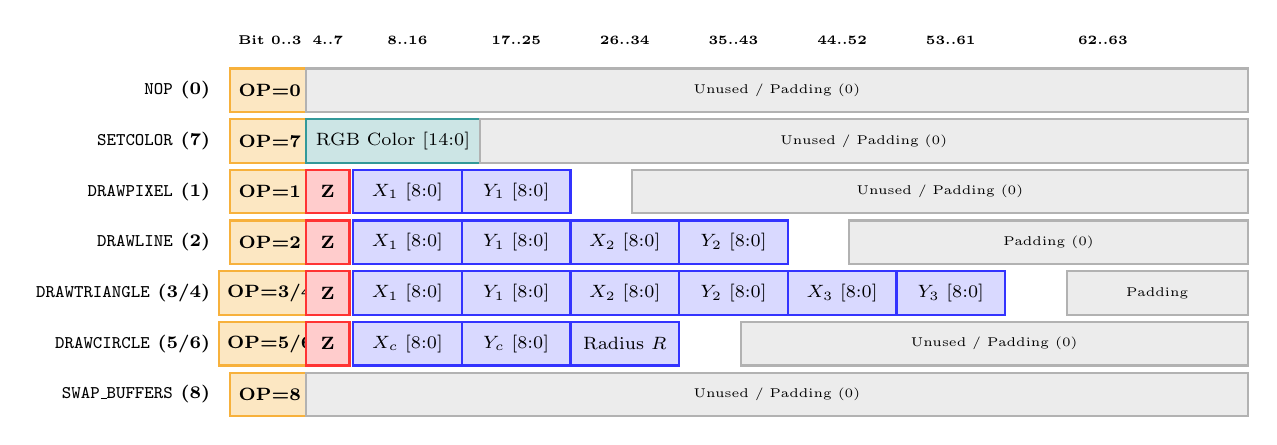
\begin{tikzpicture}[
    scale=0.92, every node/.style={transform shape},
    every text node part/.style={align=center},
    field/.style={draw=black!70, thick, fill=white, minimum height=0.6cm, font=\scriptsize},
    opfield/.style={field, fill=amber!25, draw=amber!80, font=\scriptsize\bfseries},
    zfield/.style={field, fill=red!20, draw=red!80, font=\scriptsize\bfseries},
    coordfield/.style={field, fill=blue!15, draw=blue!80},
    colorfield/.style={field, fill=teal!20, draw=teal!80},
    padfield/.style={field, fill=gray!15, draw=gray!60, font=\tiny}
]

% Bit markers on top
\node[above, font=\tiny\bfseries] at (0.5, 6.2) {Bit 0..3};
\node[above, font=\tiny\bfseries] at (1.3, 6.2) {4..7};
\node[above, font=\tiny\bfseries] at (2.4, 6.2) {8..16};
\node[above, font=\tiny\bfseries] at (3.9, 6.2) {17..25};
\node[above, font=\tiny\bfseries] at (5.4, 6.2) {26..34};
\node[above, font=\tiny\bfseries] at (6.9, 6.2) {35..43};
\node[above, font=\tiny\bfseries] at (8.4, 6.2) {44..52};
\node[above, font=\tiny\bfseries] at (9.9, 6.2) {53..61};
\node[above, font=\tiny\bfseries] at (12.0, 6.2) {62..63};

% 1. NOP
\node[left, font=\scriptsize\bfseries] at (-0.2, 5.7) {\texttt{NOP} (0)};
\node[opfield, minimum width=1.0cm] at (0.5, 5.7) {OP=0};
\node[padfield, minimum width=13.0cm] at (7.5, 5.7) {Unused / Padding (0)};

% 2. SETCOLOR
\node[left, font=\scriptsize\bfseries] at (-0.2, 5.0) {\texttt{SETCOLOR} (7)};
\node[opfield, minimum width=1.0cm] at (0.5, 5.0) {OP=7};
\node[colorfield, minimum width=2.4cm] at (2.2, 5.0) {RGB Color [14:0]};
\node[padfield, minimum width=10.6cm] at (8.7, 5.0) {Unused / Padding (0)};

% 3. DRAWPIXEL
\node[left, font=\scriptsize\bfseries] at (-0.2, 4.3) {\texttt{DRAWPIXEL} (1)};
\node[opfield, minimum width=1.0cm] at (0.5, 4.3) {OP=1};
\node[zfield, minimum width=0.6cm] at (1.3, 4.3) {Z};
\node[coordfield, minimum width=1.5cm] at (2.4, 4.3) {$X_1$ [8:0]};
\node[coordfield, minimum width=1.5cm] at (3.9, 4.3) {$Y_1$ [8:0]};
\node[padfield, minimum width=8.5cm] at (9.75, 4.3) {Unused / Padding (0)};

% 4. DRAWLINE
\node[left, font=\scriptsize\bfseries] at (-0.2, 3.6) {\texttt{DRAWLINE} (2)};
\node[opfield, minimum width=1.0cm] at (0.5, 3.6) {OP=2};
\node[zfield, minimum width=0.6cm] at (1.3, 3.6) {Z};
\node[coordfield, minimum width=1.5cm] at (2.4, 3.6) {$X_1$ [8:0]};
\node[coordfield, minimum width=1.5cm] at (3.9, 3.6) {$Y_1$ [8:0]};
\node[coordfield, minimum width=1.5cm] at (5.4, 3.6) {$X_2$ [8:0]};
\node[coordfield, minimum width=1.5cm] at (6.9, 3.6) {$Y_2$ [8:0]};
\node[padfield, minimum width=5.5cm] at (11.25, 3.6) {Padding (0)};

% 5. DRAWTRIANGLE / DRAWTRIANGLE_F
\node[left, font=\scriptsize\bfseries] at (-0.2, 2.9) {\texttt{DRAWTRIANGLE} (3/4)};
\node[opfield, minimum width=1.0cm] at (0.5, 2.9) {OP=3/4};
\node[zfield, minimum width=0.6cm] at (1.3, 2.9) {Z};
\node[coordfield, minimum width=1.5cm] at (2.4, 2.9) {$X_1$ [8:0]};
\node[coordfield, minimum width=1.5cm] at (3.9, 2.9) {$Y_1$ [8:0]};
\node[coordfield, minimum width=1.5cm] at (5.4, 2.9) {$X_2$ [8:0]};
\node[coordfield, minimum width=1.5cm] at (6.9, 2.9) {$Y_2$ [8:0]};
\node[coordfield, minimum width=1.5cm] at (8.4, 2.9) {$X_3$ [8:0]};
\node[coordfield, minimum width=1.5cm] at (9.9, 2.9) {$Y_3$ [8:0]};
\node[padfield, minimum width=2.5cm] at (12.75, 2.9) {Padding};

% 6. DRAWCIRCLE / DRAWCIRCLE_F
\node[left, font=\scriptsize\bfseries] at (-0.2, 2.2) {\texttt{DRAWCIRCLE} (5/6)};
\node[opfield, minimum width=1.0cm] at (0.5, 2.2) {OP=5/6};
\node[zfield, minimum width=0.6cm] at (1.3, 2.2) {Z};
\node[coordfield, minimum width=1.5cm] at (2.4, 2.2) {$X_c$ [8:0]};
\node[coordfield, minimum width=1.5cm] at (3.9, 2.2) {$Y_c$ [8:0]};
\node[coordfield, minimum width=1.5cm] at (5.4, 2.2) {Radius $R$};
\node[padfield, minimum width=7.0cm] at (10.5, 2.2) {Unused / Padding (0)};

% 7. SWAP_BUFFERS
\node[left, font=\scriptsize\bfseries] at (-0.2, 1.5) {\texttt{SWAP\_BUFFERS} (8)};
\node[opfield, minimum width=1.0cm] at (0.5, 1.5) {OP=8};
\node[padfield, minimum width=13.0cm] at (7.5, 1.5) {Unused / Padding (0)};

\end{tikzpicture}

}
\caption{spISA 64-Bit Instruction Word Bitfield Allocations.}
\label{fig:spisa_bitfields}
\end{figure}

\section{Bitfield Definitions and Allocations}
As defined in \texttt{sp-pkg.vhd} and illustrated in Figure~\ref{fig:spisa_bitfields}, the 64-bit instruction fields are structured as follows:
\begin{itemize}
    \item \textbf{Opcode (\texttt{OP})}: Bits \texttt{[3:0]} specify the primary operation code. An 8-bit allocation (\texttt{N\_opcode = 8}) is reserved in the hardware package to support future ISA expansions.
    \item \textbf{Depth Coordinate ($Z$)}: Bits \texttt{[7:4]} define a 4-bit unsigned depth value for geometric drawing instructions, providing 16 discrete depth sorting layers ($0 \dots 15$). A value of $Z = 0$ represents the nearest layer to the viewer, while $Z = 15$ represents the farthest background plane.
    \item \textbf{Pixel Coordinates ($X, Y$)}: Discrete spatial coordinates are encoded as 9-bit unsigned integer fields (\texttt{N\_pixel = 9}), providing an addressable coordinate space of $[0, 511]$, which naturally covers the $320 \times 240$ screen geometry.
    \item \textbf{Color Value (\texttt{Color})}: Encoded as a 15-bit RGB555 integer within bits \texttt{[22:8]} of the \texttt{SETCOLOR} instruction (5 bits Red, 5 bits Green, 5 bits Blue), capable of expressing $32{,}768$ distinct colors.
\end{itemize}

\section{Detailed Instruction Specifications}
Table~\ref{tab:spisa_summary} summarizes the complete set of supported operations in spISA.

\begin{table}[htbp]
\centering
\caption{spISA 64-Bit Instruction Set Summary}
\label{tab:spisa_summary}
\begin{tabular}{@{}cclp{7.0cm}@{}}
\toprule
\textbf{Opcode} & \textbf{Binary} & \textbf{Mnemonic} & \textbf{Functional Description and Parameters} \\ \midrule
$0$ & \texttt{0000} & \texttt{NOP} & No Operation. Propagated in broadcast to all cores. \\
$1$ & \texttt{0001} & \texttt{DRAWPIXEL} & Renders a single pixel at $(X_1, Y_1)$ with depth $Z$. \\
$2$ & \texttt{0010} & \texttt{DRAWLINE} & Renders a 1-pixel wide line segment between $(X_1, Y_1)$ and $(X_2, Y_2)$ with depth $Z$. \\
$3$ & \texttt{0011} & \texttt{DRAWTRIANGLE} & Draws the outline of a triangle with vertices $(X_1, Y_1)$, $(X_2, Y_2)$, and $(X_3, Y_3)$ with depth $Z$. \\
$4$ & \texttt{0100} & \texttt{DRAWTRIANGLE\_F} & Rasterizes a solid filled triangle with vertices $(X_1, Y_1)$, $(X_2, Y_2)$, and $(X_3, Y_3)$ with depth $Z$. \\
$5$ & \texttt{0101} & \texttt{DRAWCIRCLE} & Draws the outline of a circle centered at $(X_c, Y_c)$ with radius $R$ and depth $Z$. \\
$6$ & \texttt{0110} & \texttt{DRAWCIRCLE\_F} & Rasterizes a solid filled disk centered at $(X_c, Y_c)$ with radius $R$ and depth $Z$. \\
$7$ & \texttt{0111} & \texttt{SETCOLOR} & Updates the active 15-bit color register in all cores to the RGB555 value encoded in bits $[22:8]$. \\
$8$ & \texttt{1000} & \texttt{SWAP\_BUFFERS} & Global synchronization instruction. Triggers front/back buffer swap across all 10 tiles upon VSYNC. \\ \bottomrule
\end{tabular}
\end{table}

\subsection{Broadcast Instructions vs. Spatial Primitives}
Instructions in spISA are categorized into two fundamental operational classes:
\begin{enumerate}
    \item \textbf{Global Broadcast Instructions}: \texttt{NOP} (0), \texttt{SETCOLOR} (7), and \texttt{SWAP\_BUFFERS} (8). These instructions modify the global state of the rendering pipeline. Consequently, the hardware scheduler broadcasts these words unconditionally into the command FIFOs of all 10 compute cores simultaneously.
    \item \textbf{Spatial Drawing Primitives}: \texttt{DRAWPIXEL} (1), \texttt{DRAWLINE} (2), \texttt{DRAWTRIANGLE} (3), \texttt{DRAWTRIANGLE\_F} (4), \texttt{DRAWCIRCLE} (5), and \texttt{DRAWCIRCLE\_F} (6). These primitives describe localized 2D shapes. The scheduler computes their vertical bounding boxes and dispatches the instruction only to the specific cores whose screen tiles intersect the primitive, as elaborated in Chapter~\ref{chap:scheduler}.
\end{enumerate}

\chapter{Multicore Tiling and Spatial Parallelism}
\label{chap:multicore_tiling}

\section{Spatial Decomposition Methodology}
A primary challenge in high-performance GPU design is resolving the "memory wall"---the bottleneck where multiple parallel compute pipelines compete for read and write bandwidth to a centralized frame buffer.

To completely eliminate memory arbitration delays and bus contention, spGPU implements a \textbf{Tile-Based Spatial Partitioning} architecture. The full rendering canvas of $320 \times 240$ pixels is subdivided horizontally into 10 discrete, non-overlapping strips called \textit{Tiles}:
\begin{equation}
H_{\text{total}} = 240 \text{ lines}, \quad N_{\text{cores}} = 10 \implies H_{\text{tile}} = \frac{H_{\text{total}}}{N_{\text{cores}}} = \frac{240}{10} = 24 \text{ lines/tile}
\end{equation}

Each tile encompasses an area of $320 \times 24 = 7{,}680$ pixels. A dedicated compute core (\texttt{spCORE}) and a dedicated, isolated dual-port Block RAM memory block (\texttt{tile.vhd}) are assigned to each tile, as illustrated in Figure~\ref{fig:multicore_tiling}.

\begin{figure}[htbp]
\centering
\resizebox{0.92\textwidth}{!}{
    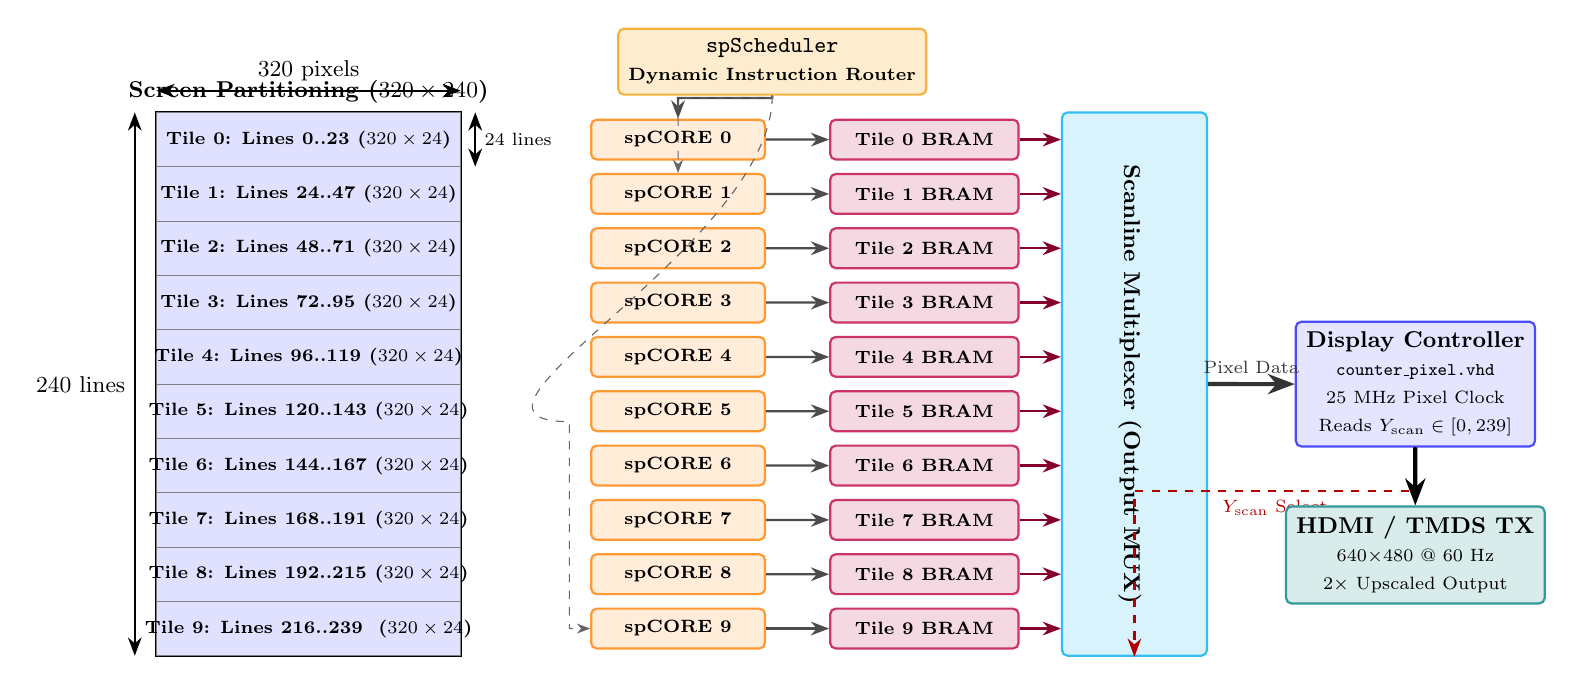
\begin{tikzpicture}[
    >=Stealth,
    scale=0.92, every node/.style={transform shape},
    every text node part/.style={align=center},
    tilelabel/.style={font=\scriptsize\bfseries},
    box/.style={draw=black!80, thick, rounded corners=2pt, fill=white, inner sep=4pt, font=\scriptsize},
    corebox/.style={box, fill=orange!15, draw=orange!80, minimum width=2.4cm, minimum height=0.55cm},
    vrambox/.style={box, fill=purple!15, draw=purple!80, minimum width=2.6cm, minimum height=0.55cm}
]

% ==================== SCREEN REPRESENTATION (320x240) ====================
\draw[thick, fill=gray!5] (0,0) rectangle (4.2, 7.5);
\node[font=\small\bfseries, above] at (2.1, 7.5) {Screen Partitioning ($320 \times 240$)};

\foreach \k/\ypos/\ystart/\yend in {
    0/6.75/0/23, 
    1/6.0/24/47, 
    2/5.25/48/71, 
    3/4.5/72/95, 
    4/3.75/96/119, 
    5/3.0/120/143, 
    6/2.25/144/167, 
    7/1.5/168/191, 
    8/0.75/192/215, 
    9/0.0/216/239
} {
    \draw[fill=blue!12, draw=black!50] (0, \ypos) rectangle (4.2, \ypos+0.75);
    \node[tilelabel] at (2.1, \ypos+0.375) {Tile \k: Lines \ystart..\yend\ ($320\times 24$)};
}

% Dimension arrows
\draw[<->, thick] (-0.3, 0) -- (-0.3, 7.5) node[midway, left, font=\small] {240 lines};
\draw[<->, thick] (0, 7.8) -- (4.2, 7.8) node[midway, above, font=\small] {320 pixels};
\draw[<->, thick] (4.4, 6.75) -- (4.4, 7.5) node[midway, right, font=\scriptsize] {24 lines};

% ==================== SCHEDULER ====================
\node[box, fill=amber!20, draw=amber!80, minimum width=3.2cm, font=\small\bfseries] (sched) at (8.5, 8.2) {
    \texttt{spScheduler}\\
    \scriptsize Dynamic Instruction Router
};

% ==================== CORES AND MEMORIES ====================
\foreach \k/\ypos in {
    0/6.75, 1/6.0, 2/5.25, 3/4.5, 4/3.75, 5/3.0, 6/2.25, 7/1.5, 8/0.75, 9/0.0
} {
    \node[corebox] (core\k) at (7.2, \ypos+0.375) {\textbf{spCORE \k}};
    \node[vrambox] (vram\k) at (10.6, \ypos+0.375) {\textbf{Tile \k\ BRAM}};
    
    % Core to VRAM connection
    \draw[->, thick, black!70] (core\k) -- (vram\k);
}

% Draw scheduler distribution bus
\draw[->, thick, black!70] (sched.south) -- (8.5, 7.7) -| (core0.north);
\draw[->, dashed, black!60] (sched.south) -- (8.5, 7.7) -| (core1.north);
\draw[->, dashed, black!60] (sched.south) to[out=-90, in=180] ++(-2.8, -4.5) |- (core9.west);

% ==================== SCANLINE MULTIPLEXER ====================
\node[box, fill=cyan!15, draw=cyan!80, minimum width=2.0cm, minimum height=7.5cm, font=\small\bfseries] (mux) at (13.5, 3.75) {
    \rotatebox{-90}{Scanline Multiplexer (Output MUX)}
};

\foreach \k in {0,1,2,3,4,5,6,7,8,9} {
    \draw[->, thick, purple!70!black] (vram\k.east) -- (vram\k.east -| mux.west);
}

% ==================== VIDEO CONTROLLER ====================
\node[box, fill=blue!10, draw=blue!70, right=1.2cm of mux, font=\small] (disp) {
    \textbf{Display Controller}\\
    \scriptsize\texttt{counter\_pixel.vhd}\\
    \scriptsize 25 MHz Pixel Clock\\
    \scriptsize Reads $Y_{\text{scan}} \in [0, 239]$
};
\draw[->, line width=1.5pt, black!80] (mux.east) -- node[above, font=\scriptsize] {Pixel Data} (disp.west);
\draw[->, thick, dashed, red!70!black] (disp.south) -- ++(0,-0.6) -| node[pos=0.25, below, font=\scriptsize] {$Y_{\text{scan}}$ Select} (mux.south);

% ==================== HDMI OUTPUT ====================
\node[box, fill=teal!15, draw=teal!80, below=0.8cm of disp, font=\small] (hdmi) {
    \textbf{HDMI / TMDS TX}\\
    \scriptsize 640$\times$480 @ 60 Hz\\
    \scriptsize $2\times$ Upscaled Output
};
\draw[->, line width=1.5pt] (disp) -- (hdmi);

\end{tikzpicture}

}
\caption{spGPU Multicore Spatial Tiling and Display Scanning Architecture.}
\label{fig:multicore_tiling}
\end{figure}

\section{Core-to-Tile Mapping and Coordinate Spaces}
Each core $i \in [0, 9]$ operates on global coordinates during instruction decode, but writes exclusively into its local $320 \times 24$ tile VRAM. The vertical start offset of each tile is precomputed at compile time by the deferred constant function \texttt{calc\_y\_tile\_start} in \texttt{sp-pkg.vhd}:
\begin{equation}
Y_{\text{tile\_start}}(i) = i \times 24
\end{equation}

Table~\ref{tab:tiling_map} specifies the physical mapping between cores, tiles, scanlines, and memory allocations.

\begin{table}[htbp]
\centering
\caption{Multicore Tile Mapping and Memory Footprint}
\label{tab:tiling_map}
\begin{tabular}{@{}ccccc@{}}
\toprule
\textbf{Core ID} & \textbf{Assigned Tile} & \textbf{Global $Y$ Scanlines} & \textbf{Local $Y$ Range} & \textbf{VRAM Footprint ($2\times$ Buffer)} \\ \midrule
\texttt{spCORE 0} & Tile 0 & $0 \dots 23$   & $0 \dots 23$ & $15{,}360 \times 15$-bit ($230.4\text{ kb}$) \\
\texttt{spCORE 1} & Tile 1 & $24 \dots 47$  & $0 \dots 23$ & $15{,}360 \times 15$-bit ($230.4\text{ kb}$) \\
\texttt{spCORE 2} & Tile 2 & $48 \dots 71$  & $0 \dots 23$ & $15{,}360 \times 15$-bit ($230.4\text{ kb}$) \\
\texttt{spCORE 3} & Tile 3 & $72 \dots 95$  & $0 \dots 23$ & $15{,}360 \times 15$-bit ($230.4\text{ kb}$) \\
\texttt{spCORE 4} & Tile 4 & $96 \dots 119$ & $0 \dots 23$ & $15{,}360 \times 15$-bit ($230.4\text{ kb}$) \\
\texttt{spCORE 5} & Tile 5 & $120 \dots 143$ & $0 \dots 23$ & $15{,}360 \times 15$-bit ($230.4\text{ kb}$) \\
\texttt{spCORE 6} & Tile 6 & $144 \dots 167$ & $0 \dots 23$ & $15{,}360 \times 15$-bit ($230.4\text{ kb}$) \\
\texttt{spCORE 7} & Tile 7 & $168 \dots 191$ & $0 \dots 23$ & $15{,}360 \times 15$-bit ($230.4\text{ kb}$) \\
\texttt{spCORE 8} & Tile 8 & $192 \dots 215$ & $0 \dots 23$ & $15{,}360 \times 15$-bit ($230.4\text{ kb}$) \\
\texttt{spCORE 9} & Tile 9 & $216 \dots 239$ & $0 \dots 23$ & $15{,}360 \times 15$-bit ($230.4\text{ kb}$) \\ \midrule
\textbf{Total} & \textbf{10 Tiles} & \textbf{0 \dots 239} & \textbf{--} & \textbf{153{,}600 words ($\approx 2.30\text{ Mb}$)} \\ \bottomrule
\end{tabular}
\end{table}

\section{Throughput Scaling and Hardware Benefits}
The architectural benefits of this spatial partitioning are significant:
\begin{enumerate}
    \item \textbf{True Parallel Memory Writes}: At any given clock cycle, all 10 cores can execute write operations simultaneously into their respective BRAM blocks. There are no shared arbiter stalls, crossbar multiplexers, or wait states on the write ports.
    \item \textbf{Near-Linear Acceleration for Distributed Scenes}: When drawing objects that span multiple vertical regions of the display (such as the 10 bouncing spheres in the demo application), all 10 cores compute concurrently, yielding up to a $10\times$ speedup compared to a single-core implementation.
    \item \textbf{Decoupled Display Readout}: The display controller reads sequential scanlines for video generation using Port B of the dual-port RAMs. Because each tile is an independent memory primitive, the video controller reads from only one tile at a time via the output multiplexer, while all 10 cores continue writing freely to their respective Port A interfaces.
\end{enumerate}

\chapter{Dynamic Instruction Scheduler}
\label{chap:scheduler}

\section{Role and Motivation of the Scheduler}
In a tiled multicore graphics architecture, broadcasting every drawing instruction unconditionally to every core would force all cores to compute all primitives, defeating the purpose of spatial parallelism and wasting power and clock cycles.

The \textbf{\texttt{spScheduler}} component acts as an intelligent hardware router. It receives the incoming stream of 64-bit instructions from the AXI-Stream interface, evaluates the geometric vertical boundaries of the target primitive in single-cycle combinatorial logic, and selectively dispatches the instruction word \textit{only} to the FIFOs of the cores whose tile areas physically intersect the shape.

Figure~\ref{fig:scheduler} depicts the internal block diagram of the dynamic scheduler, including the pre-decode bounding box logic, the range classifier, the FIFO bank, and the backpressure flow control.

\begin{figure}[htbp]
\centering
\resizebox{0.95\textwidth}{!}{
    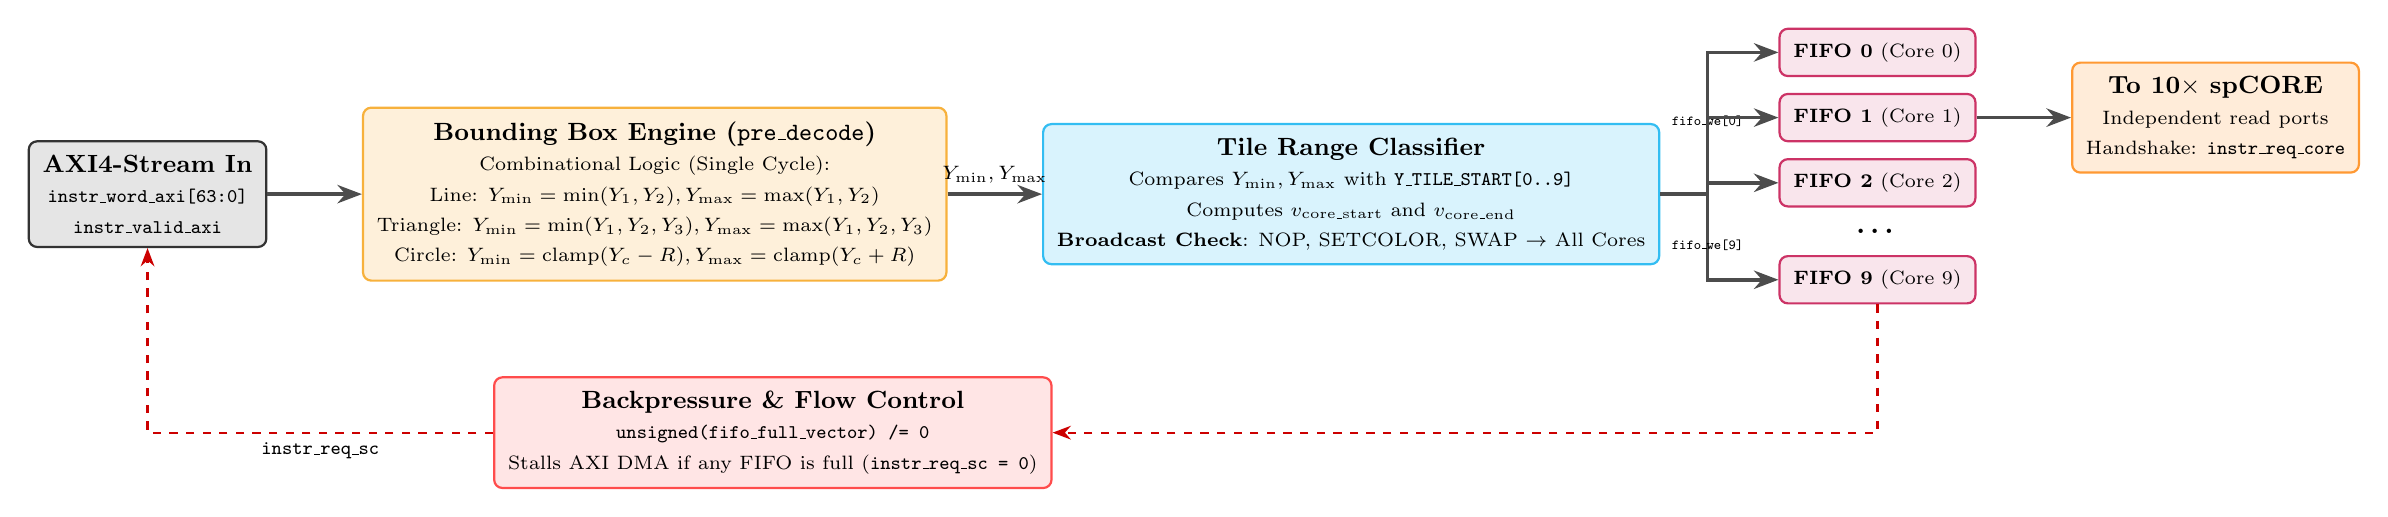
\begin{tikzpicture}[
    >=Stealth,
    node distance=1.0cm and 1.2cm,
    every text node part/.style={align=center},
    box/.style={draw=black!80, thick, rounded corners=3pt, fill=white, inner sep=5pt, font=\small},
    logicbox/.style={box, fill=amber!15, draw=amber!80, minimum width=3.4cm},
    fifobox/.style={box, fill=purple!10, draw=purple!80, minimum width=2.4cm, minimum height=0.6cm, font=\scriptsize},
    bus/.style={draw=black!70, line width=1.3pt, ->},
    sig/.style={draw=blue!70!black, thick, ->},
    ctl/.style={draw=red!80!black, dashed, thick, ->}
]

% ==================== INPUT INSTRUCTION ====================
\node[box, fill=gray!20] (axi_in) {
    \textbf{AXI4-Stream In}\\
    \scriptsize\texttt{instr\_word\_axi[63:0]}\\
    \scriptsize\texttt{instr\_valid\_axi}
};

% ==================== BOUNDING BOX DECODER ====================
\node[logicbox, right=1.2cm of axi_in] (bbox_unit) {
    \textbf{Bounding Box Engine (\texttt{pre\_decode})}\\
    \scriptsize Combinational Logic (Single Cycle):\\
    \scriptsize Line: $Y_{\min} = \min(Y_1,Y_2), Y_{\max} = \max(Y_1,Y_2)$\\
    \scriptsize Triangle: $Y_{\min} = \min(Y_1,Y_2,Y_3), Y_{\max} = \max(Y_1,Y_2,Y_3)$\\
    \scriptsize Circle: $Y_{\min} = \text{clamp}(Y_c - R), Y_{\max} = \text{clamp}(Y_c + R)$
};
\draw[bus] (axi_in) -- (bbox_unit);

% ==================== TILE RANGE MAPPER ====================
\node[logicbox, fill=cyan!15, draw=cyan!80, right=1.2cm of bbox_unit] (range_mapper) {
    \textbf{Tile Range Classifier}\\
    \scriptsize Compares $Y_{\min}, Y_{\max}$ with \texttt{Y\_TILE\_START[0..9]}\\
    \scriptsize Computes $v_{\text{core\_start}}$ and $v_{\text{core\_end}}$\\
    \scriptsize\textbf{Broadcast Check}: NOP, SETCOLOR, SWAP $\to$ All Cores
};
\draw[bus] (bbox_unit) -- node[above, font=\scriptsize] {$Y_{\min}, Y_{\max}$} (range_mapper);

% ==================== FIFO ARRAY ====================
\node[fifobox, right=1.5cm of range_mapper, yshift=1.8cm] (fifo0) {\textbf{FIFO 0} (Core 0)};
\node[fifobox, below=0.2cm of fifo0] (fifo1) {\textbf{FIFO 1} (Core 1)};
\node[fifobox, below=0.2cm of fifo1] (fifo2) {\textbf{FIFO 2} (Core 2)};
\node[font=\bfseries, below=0.15cm of fifo2] (fdots) {\dots};
\node[fifobox, below=0.15cm of fdots] (fifo9) {\textbf{FIFO 9} (Core 9)};

\draw[bus] (range_mapper.east) -- ++(0.6,0) |- node[pos=0.2, above, font=\tiny] {\texttt{fifo\_we[0]}} (fifo0.west);
\draw[bus] (range_mapper.east) -- ++(0.6,0) |- (fifo1.west);
\draw[bus] (range_mapper.east) -- ++(0.6,0) |- (fifo2.west);
\draw[bus] (range_mapper.east) -- ++(0.6,0) |- node[pos=0.2, below, font=\tiny] {\texttt{fifo\_we[9]}} (fifo9.west);

% ==================== BACKPRESSURE & READY GENERATION ====================
\node[box, fill=red!10, draw=red!70, below=1.2cm of bbox_unit, xshift=1.5cm, minimum width=4.5cm] (backpress) {
    \textbf{Backpressure \& Flow Control}\\
    \scriptsize \texttt{unsigned(fifo\_full\_vector) /= 0}\\
    \scriptsize Stalls AXI DMA if any FIFO is full (\texttt{instr\_req\_sc = 0})
};

\draw[ctl] (fifo9.south) |- (backpress.east);
\draw[ctl] (backpress.west) -| node[pos=0.25, below, font=\scriptsize] {\texttt{instr\_req\_sc}} (axi_in.south);

% ==================== OUTPUT TO CORES ====================
\node[box, fill=orange!15, draw=orange!80, right=1.2cm of fifo1] (to_cores) {
    \textbf{To 10$\times$ spCORE}\\
    \scriptsize Independent read ports\\
    \scriptsize Handshake: \texttt{instr\_req\_core}
};
\draw[bus] (fifo1.east) -- (to_cores.west);

\end{tikzpicture}

}
\caption{Dynamic Instruction Scheduler (\texttt{spScheduler}) Microarchitecture.}
\label{fig:scheduler}
\end{figure}

\section{Combinatorial Bounding Box Pre-Decoder}
During the \texttt{request} state, the process \texttt{pre\_decode} inspects the incoming opcode and vertex coordinates in purely combinational logic to determine the vertical interval $[Y_{\min}, Y_{\max}]$:
\begin{itemize}
    \item \textbf{Pixel (\texttt{DRAWPIXEL})}:
    \begin{equation}
    Y_{\min} = Y_1, \quad Y_{\max} = Y_1
    \end{equation}
    \item \textbf{Line (\texttt{DRAWLINE})}:
    \begin{equation}
    Y_{\min} = \min(Y_1, Y_2), \quad Y_{\max} = \max(Y_1, Y_2)
    \end{equation}
    \item \textbf{Triangles (\texttt{DRAWTRIANGLE} and \texttt{DRAWTRIANGLE\_F})}:
    \begin{equation}
    Y_{\min} = \min(Y_1, \min(Y_2, Y_3)), \quad Y_{\max} = \max(Y_1, \max(Y_2, Y_3))
    \end{equation}
    \item \textbf{Circles (\texttt{DRAWCIRCLE} and \texttt{DRAWCIRCLE\_F})}:
    Because circular geometry can extend partially off-screen, the bounding box evaluation incorporates explicit hardware clamping to prevent unsigned underflow or overflow beyond the screen height ($240$):
    \begin{equation}
    Y_{\max} = \begin{cases} 
    239 & \text{if } Y_c > (240 - R) \\ 
    Y_c + R & \text{otherwise} 
    \end{cases}
    \end{equation}
    \begin{equation}
    Y_{\min} = \begin{cases} 
    0 & \text{if } Y_c < R \\ 
    Y_c - R & \text{otherwise} 
    \end{cases}
    \end{equation}
\end{itemize}

\section{Core Range Classification and Selective Dispatching}
Once $[Y_{\min}, Y_{\max}]$ is computed, the scheduler evaluates the tile interval $[v_{\text{core\_start}}, v_{\text{core\_end}}]$ by comparing the bounds against the constant array \texttt{Y\_TILE\_START}:
\begin{lstlisting}[language=VHDL, caption={Core Range Classification Logic in \texttt{spScheduler.vhd}.}, label={lst:sched_range}]
v_core_start := 0;
v_core_end   := 0;

for i in 0 to N_cores-1 loop
    if unsigned(y_min) >= Y_TILE_START(i) then 
        v_core_start := i; 
    end if;
    if unsigned(y_max) >= Y_TILE_START(i) then 
        v_core_end := i; 
    end if;
end loop;

if v_core_start > v_core_end then
    v_core_end := v_core_start;
end if;
\end{lstlisting}

Based on this range, the scheduler directs writes to the command FIFOs:
\begin{itemize}
    \item \textbf{Broadcast Commands} (\texttt{NOP}, \texttt{SETCOLOR}, \texttt{SWAP\_BUFFERS}): The write enable signal \texttt{fifo\_we\_vector(i)} is asserted for \textbf{all 10 FIFOs}.
    \item \textbf{Drawing Primitives}: The write enable is asserted \textbf{only for cores $i \in [v_{\text{core\_start}}, v_{\text{core\_end}}]$}. All other FIFOs receive write enable \texttt{'0'}.
\end{itemize}

\section{Dedicated Synchronous FIFOs and Flow Control}
Each core is backed by an independent synchronous FIFO (\texttt{sc\_fifo.vhd}) with a parameterized depth (\texttt{FIFO\_DEPTH = 12} to $32$). These queues buffer instructions, allowing cores that finish small primitives rapidly to proceed without waiting for cores engaged in rasterizing large triangles or filled circles.

\subsection{Backpressure Mechanism}
To guarantee that fast bursts of DMA transfers never overwrite unread FIFO entries, the scheduler aggregates the full status of all 10 FIFOs:
\begin{equation}
\texttt{instr\_req\_sc} = \begin{cases} 
\text{'1'} & \text{if } (\text{state} = \texttt{request}) \land \left(\sum_{i=0}^{9} \texttt{fifo\_full}(i) = 0\right) \\ 
\text{'0'} & \text{otherwise} 
\end{cases}
\end{equation}
If any FIFO in the system becomes full, the scheduler immediately deasserts \texttt{instr\_req\_sc}, causing the upstream AXI4-Stream interface to lower \texttt{s\_axis\_tready}, effectively pausing the DMA transfer until queue space becomes available.

\chapter{Single-Core Microarchitecture (\texttt{spCORE})}
\label{chap:core_microarchitecture}

\section{Structural Overview of the Compute Core}
Each of the ten identical graphics processing units (\textbf{\texttt{spCORE}}) instantiated in the top-level entity is designed as a modular, decoupled processing engine. As shown in Figure~\ref{fig:single_core}, \texttt{spCORE} is internally divided into two primary sub-blocks:
\begin{enumerate}
    \item \textbf{\texttt{spPIPE}} (\textit{Instruction Pipeline, Fetch, Decode \& Registers}): Manages the core command interface, decodes 64-bit spISA words, latches vertex and color parameters into dedicated registers, and orchestrates the core execution state machine.
    \item \textbf{\texttt{spEXEC}} (\textit{Execution Unit, Dedicated Accelerators \& Tile Boundary Protection}): Houses the parallel hardware rasterization engines, arbitrates the generated pixel streams, handles swap handshaking, and enforces hard spatial clipping boundaries for the tile.
\end{enumerate}

\begin{figure}[htbp]
\centering
\resizebox{0.95\textwidth}{!}{
    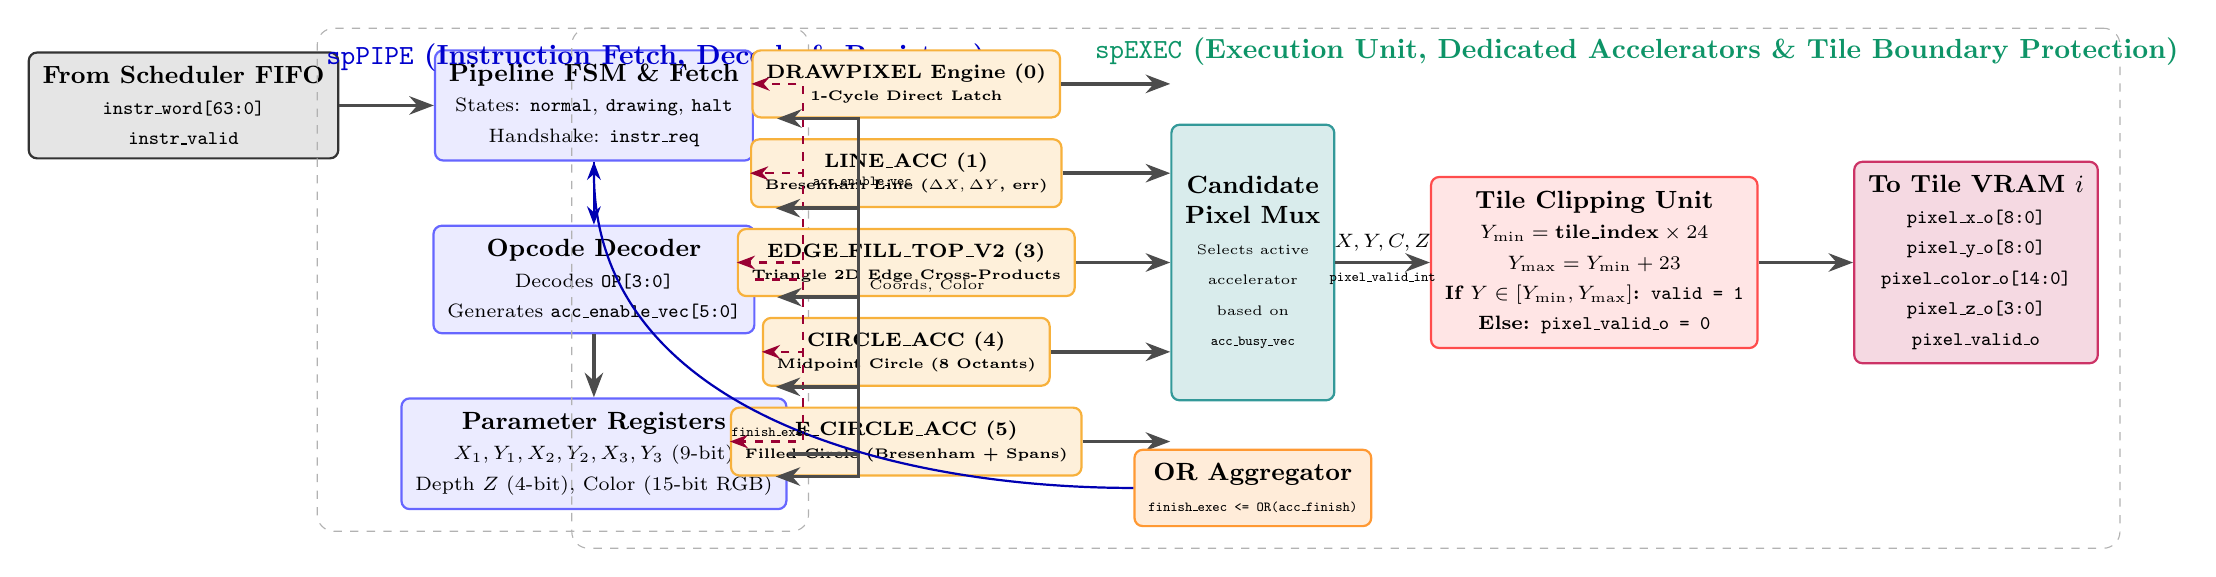
\begin{tikzpicture}[
    >=Stealth,
    node distance=1.0cm and 1.2cm,
    every text node part/.style={align=center},
    box/.style={draw=black!80, thick, rounded corners=3pt, fill=white, inner sep=5pt, font=\small},
    pipebox/.style={box, fill=blue!8, draw=blue!60},
    execbox/.style={box, fill=emerald!8, draw=emerald!60},
    accbox/.style={box, fill=amber!15, draw=amber!80, minimum width=2.6cm, minimum height=0.75cm, font=\scriptsize\bfseries},
    clipbox/.style={box, fill=red!10, draw=red!70, font=\small\bfseries},
    bus/.style={draw=black!70, line width=1.3pt, ->},
    sig/.style={draw=blue!70!black, thick, ->},
    ctl/.style={draw=purple!80!black, dashed, thick, ->},
    subframe/.style={draw=gray!60, dashed, rounded corners=6pt, inner sep=8pt}
]

% ==================== spCORE INPUTS ====================
\node[box, fill=gray!20] (in_fifo) {
    \textbf{From Scheduler FIFO}\\
    \scriptsize\texttt{instr\_word[63:0]}\\
    \scriptsize\texttt{instr\_valid}
};

% ==================== spPIPE UNIT ====================
\begin{scope}[local bounding box=pipe_unit]
    \node[pipebox, right=1.2cm of in_fifo, minimum width=3.4cm] (fsm_fetch) {
        \textbf{Pipeline FSM \& Fetch}\\
        \scriptsize States: \texttt{normal}, \texttt{drawing}, \texttt{halt}\\
        \scriptsize Handshake: \texttt{instr\_req}
    };

    \node[pipebox, below=0.8cm of fsm_fetch, minimum width=3.4cm] (decoder) {
        \textbf{Opcode Decoder}\\
        \scriptsize Decodes \texttt{OP[3:0]}\\
        \scriptsize Generates \texttt{acc\_enable\_vec[5:0]}
    };

    \node[pipebox, below=0.8cm of decoder, minimum width=3.4cm] (param_regs) {
        \textbf{Parameter Registers}\\
        \scriptsize $X_1, Y_1, X_2, Y_2, X_3, Y_3$ (9-bit)\\
        \scriptsize Depth $Z$ (4-bit), Color (15-bit RGB)
    };

    \draw[bus] (in_fifo) -- (fsm_fetch);
    \draw[sig] (fsm_fetch) -- (decoder);
    \draw[bus] (decoder) -- (param_regs);
\end{scope}
\node[subframe, fit=(pipe_unit), label={[anchor=north west, font=\bfseries\color{blue!80!black}]above left:\texttt{spPIPE} (Instruction Fetch, Decode \& Registers)}] {};

% ==================== ACCELERATORS (in spEXEC) ====================
\begin{scope}[local bounding box=acc_array]
    \node[accbox, right=2.0cm of fsm_fetch.north, anchor=north west] (acc_pixel) {
        DRAWPIXEL Engine (0)\\
        \tiny 1-Cycle Direct Latch
    };
    \node[accbox, below=0.25cm of acc_pixel] (acc_line) {
        LINE\_ACC (1)\\
        \tiny Bresenham Line ($\Delta X, \Delta Y$, err)
    };
    \node[accbox, below=0.25cm of acc_line] (acc_tri) {
        EDGE\_FILL\_TOP\_V2 (3)\\
        \tiny Triangle 2D Edge Cross-Products
    };
    \node[accbox, below=0.25cm of acc_tri] (acc_circ) {
        CIRCLE\_ACC (4)\\
        \tiny Midpoint Circle (8 Octants)
    };
    \node[accbox, below=0.25cm of acc_circ] (acc_fcirc) {
        F\_CIRCLE\_ACC (5)\\
        \tiny Filled Circle (Bresenham + Spans)
    };
\end{scope}

% Routing from spPIPE to Accelerators
\draw[ctl] (decoder.east) -- ++(0.6,0) |- node[pos=0.25, right, font=\tiny] {\texttt{acc\_enable\_vec}} (acc_pixel.west);
\draw[ctl] (decoder.east) -- ++(0.6,0) |- (acc_line.west);
\draw[ctl] (decoder.east) -- ++(0.6,0) |- (acc_tri.west);
\draw[ctl] (decoder.east) -- ++(0.6,0) |- (acc_circ.west);
\draw[ctl] (decoder.east) -- ++(0.6,0) |- (acc_fcirc.west);

\draw[bus] (param_regs.east) -- ++(0.9,0) |- node[pos=0.25, right, font=\tiny] {Coords, Color} (acc_pixel.195);
\draw[bus] (param_regs.east) -- ++(0.9,0) |- (acc_line.195);
\draw[bus] (param_regs.east) -- ++(0.9,0) |- (acc_tri.195);
\draw[bus] (param_regs.east) -- ++(0.9,0) |- (acc_circ.195);
\draw[bus] (param_regs.east) -- ++(0.9,0) |- (acc_fcirc.195);

% ==================== EXECUTION & ARBITRATION ====================
\begin{scope}[local bounding box=exec_tail]
    % Pixel Multiplexer
    \node[box, fill=teal!15, draw=teal!80, right=1.2cm of acc_tri, minimum height=3.5cm, minimum width=1.6cm] (mux_pixel) {
        \textbf{Candidate}\\
        \textbf{Pixel Mux}\\
        \tiny Selects active\\
        \tiny accelerator\\
        \tiny based on\\
        \tiny\texttt{acc\_busy\_vec}
    };

    \draw[bus] (acc_pixel.east) -- (acc_pixel.east -| mux_pixel.west);
    \draw[bus] (acc_line.east) -- (acc_line.east -| mux_pixel.west);
    \draw[bus] (acc_tri.east) -- (mux_pixel.west);
    \draw[bus] (acc_circ.east) -- (acc_circ.east -| mux_pixel.west);
    \draw[bus] (acc_fcirc.east) -- (acc_fcirc.east -| mux_pixel.west);

    % Completion OR Gate
    \node[box, fill=orange!15, draw=orange!80, below=0.6cm of mux_pixel, minimum width=2.2cm] (or_finish) {
        \textbf{OR Aggregator}\\
        \tiny\texttt{finish\_exec <= OR(acc\_finish)}
    };
    \draw[sig] (or_finish.west) to[out=180, in=-90] node[below, font=\tiny] {\texttt{finish\_exec}} (fsm_fetch.south);

    % Hardware Tile Clipping Unit
    \node[clipbox, right=1.2cm of mux_pixel, minimum width=3.4cm, minimum height=1.6cm] (clip_unit) {
        \textbf{Tile Clipping Unit}\\
        \scriptsize $Y_{\min} = \text{tile\_index} \times 24$\\
        \scriptsize $Y_{\max} = Y_{\min} + 23$\\
        \scriptsize If $Y \in [Y_{\min}, Y_{\max}]$: \texttt{valid = 1}\\
        \scriptsize Else: \texttt{pixel\_valid\_o = 0}
    };
    \draw[bus] (mux_pixel) -- node[above, font=\scriptsize] {$X, Y, C, Z$} node[below, font=\tiny] {\texttt{pixel\_valid\_int}} (clip_unit);

    \node[box, fill=purple!15, draw=purple!80, right=1.2cm of clip_unit] (out_tile) {
        \textbf{To Tile VRAM $i$}\\
        \scriptsize\texttt{pixel\_x\_o[8:0]}\\
        \scriptsize\texttt{pixel\_y\_o[8:0]}\\
        \scriptsize\texttt{pixel\_color\_o[14:0]}\\
        \scriptsize\texttt{pixel\_z\_o[3:0]}\\
        \scriptsize\texttt{pixel\_valid\_o}
    };
    \draw[bus] (clip_unit) -- (out_tile);
\end{scope}

\node[subframe, fit=(acc_array) (exec_tail), label={[anchor=north west, font=\bfseries\color{emerald!80!black}]above left:\texttt{spEXEC} (Execution Unit, Dedicated Accelerators \& Tile Boundary Protection)}] {};

\end{tikzpicture}

}
\caption{Microarchitecture of the Single Graphics Core (\texttt{spCORE}).}
\label{fig:single_core}
\end{figure}

\section{Pipeline Control and Decode Unit (\texttt{spPIPE.vhd})}
The \texttt{spPIPE} block is responsible for synchronizing instruction ingestion with accelerator availability.

\subsection{Pipeline Finite State Machine}
The pipeline controller is governed by an FSM with three operational states:
\begin{itemize}
    \item \texttt{normal}: The core asserts \texttt{instr\_req <= '1'} toward its dedicated scheduler FIFO. When \texttt{instr\_valid} is sampled high, the 64-bit instruction word is latched. The opcode decoder evaluates bits \texttt{[3:0]}:
    \begin{itemize}
        \item If \texttt{NOP}, parameters are cleared and the core remains in \texttt{normal}.
        \item If \texttt{SETCOLOR}, the 15-bit color field is stored in the internal color register \texttt{color\_int} and the state remains \texttt{normal}.
        \item If a drawing primitive or \texttt{SWAP\_BUFFERS} is detected, the corresponding accelerator enable line in \texttt{acc\_enable\_vec[5:0]} is pulsed, the busy mask \texttt{acc\_busy\_vec} is set, and the FSM transitions to \texttt{drawing}.
    \end{itemize}
    \item \texttt{drawing}: In this state, \texttt{instr\_req} is held low to stall further instruction fetching. The core remains in \texttt{drawing} until the execution unit signals completion via \texttt{finish\_exec = '1'}, at which point the state transitions back to \texttt{normal}.
    \item \texttt{halt}: An asynchronous stall state entered whenever the external signal \texttt{core\_halt} is asserted.
\end{itemize}

\subsection{Parameter Registration}
During decode, the packed bitfields of the instruction word are extracted and registered into dedicated 9-bit coordinate buses: $(X_1, Y_1)$, $(X_2, Y_2)$, $(X_3, Y_3)$, depth $Z$, and the active 15-bit RGB color.

\section{Execution Unit and Tile Boundary Protection (\texttt{spEXEC.vhd})}
The \texttt{spEXEC} module interfaces the control signals from \texttt{spPIPE} to the physical rasterization engines.

\subsection{Candidate Pixel Multiplexing and Completion Aggregation}
When a drawing primitive is active, its corresponding hardware accelerator outputs a continuous stream of candidate pixels $(X, Y, \text{Color})$ qualified by an individual \texttt{pixel\_valid} flag. The multiplexer process \texttt{pixel\_out\_proc} routes the active accelerator's outputs to the internal bus based on \texttt{acc\_busy\_vec}.

Simultaneously, the completion signals from all six accelerators and the swap controller are logically OR-ed to generate \texttt{finish\_exec}:
\begin{equation}
\texttt{finish\_exec} = \bigvee_{k=0}^{5} \texttt{acc\_finish\_vec}(k) \lor \texttt{finish\_swap}
\end{equation}
This single-cycle pulse informs \texttt{spPIPE} that the primitive has been completely rasterized, allowing the core to fetch the next instruction from its FIFO.

\subsection{Hardware Tile Clipping Unit}
While the upstream scheduler restricts instruction dispatch to overlapping tiles, primitives that cross multiple tiles will naturally produce pixels outside the vertical bounds of any single tile. 

To prevent out-of-bounds pixels from contaminating adjacent tile memory blocks or causing address wrap-around, \texttt{spEXEC} implements a dedicated, zero-latency \textbf{Tile Clipping Process} (\texttt{pixel\_clip\_proc}):
\begin{lstlisting}[language=VHDL, caption={Tile Boundary Enforcement in \texttt{spEXEC.vhd}.}, label={lst:tile_clipping}]
pixel_clip_proc : process(pixel_x_int, pixel_y_int, pixel_color_int, z_i, pixel_valid_int, tile_index)
    variable x_coord, y_coord : integer;
    variable y_min, y_max     : integer;
begin
    x_coord := to_integer(unsigned(pixel_x_int));
    y_coord := to_integer(unsigned(pixel_y_int));
    
    y_min := to_integer(unsigned(tile_index)) * 24;
    y_max := y_min + 23;
    
    pixel_x_o     <= pixel_x_int;
    pixel_y_o     <= pixel_y_int;
    pixel_color_o <= pixel_color_int;
    pixel_z_o     <= z_i;
    
    if pixel_valid_int = '1' then
        if (x_coord >= 0 and x_coord < 320) and (y_coord >= y_min and y_coord <= y_max) then
            pixel_valid_o <= '1';
        else
            pixel_valid_o <= '0'; -- Zero-overhead hardware suppression
        end if;
    else
        pixel_valid_o <= '0';
    end if;
end process pixel_clip_proc;
\end{lstlisting}

If a candidate pixel's $Y$ coordinate satisfies $Y \in [i \times 24, i \times 24 + 23]$, it is written into VRAM. If it falls outside this 24-line boundary, \texttt{pixel\_valid\_o} is driven to \texttt{'0'}, silently discarding the pixel without interrupting the accelerator pipeline.

\chapter{Hardware Primitive Accelerators}
\label{chap:hardware_accelerators}

\section{Overview of Dedicated Acceleration Engines}
The core computational strength of spGPU resides in its suite of specialized, integer-arithmetic hardware accelerators instantiated within each \texttt{spCORE}. Rather than relying on a general-purpose ALU to execute iterative software rasterization loops, these units are synthesized directly as dedicated finite state machines and data-path pipelines.

Figure~\ref{fig:accelerators} presents the internal mathematical structures and operational data paths of the key acceleration engines.

\begin{figure}[htbp]
\centering
\resizebox{0.95\textwidth}{!}{
    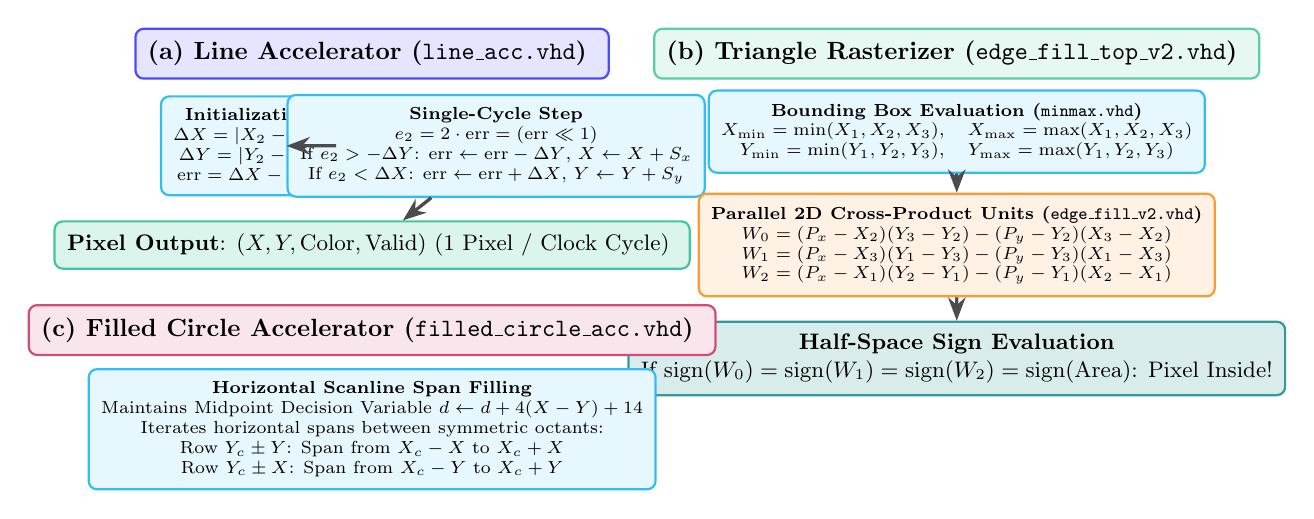
\begin{tikzpicture}[
    >=Stealth,
    scale=0.9, every node/.style={transform shape},
    every text node part/.style={align=center},
    box/.style={draw=black!80, thick, rounded corners=3pt, fill=white, inner sep=5pt, font=\small},
    accbox/.style={box, fill=amber!10, draw=amber!80},
    mathnode/.style={box, fill=cyan!10, draw=cyan!80, font=\scriptsize},
    bus/.style={draw=black!70, line width=1.2pt, ->}
]

% ==================== SUBFIGURE A: BRESENHAM LINE ====================
\node[accbox, font=\bfseries, minimum width=6.5cm, fill=blue!10, draw=blue!70] (title_line) at (3.25, 6.5) {
    (a) Line Accelerator (\texttt{line\_acc.vhd})
};

\node[mathnode] (line_init) at (1.5, 5.2) {
    \textbf{Initialization}\\
    $\Delta X = |X_2 - X_1|$\\
    $\Delta Y = |Y_2 - Y_1|$\\
    $\text{err} = \Delta X - \Delta Y$
};

\node[mathnode] (line_iter) at (5.0, 5.2) {
    \textbf{Single-Cycle Step}\\
    $e_2 = 2 \cdot \text{err} = (\text{err} \ll 1)$\\
    If $e_2 > -\Delta Y$: $\text{err} \gets \text{err} - \Delta Y$, $X \gets X + S_x$\\
    If $e_2 < \Delta X$: $\text{err} \gets \text{err} + \Delta X$, $Y \gets Y + S_y$
};

\node[box, fill=emerald!15, draw=emerald!80] (line_out) at (3.25, 3.8) {
    \textbf{Pixel Output}: $(X, Y, \text{Color}, \text{Valid})$ (1 Pixel / Clock Cycle)
};

\draw[bus] (line_init) -- (line_iter);
\draw[bus] (line_iter) -- (line_out);

% ==================== SUBFIGURE B: TRIANGLE EDGE CROSS PRODUCTS ====================
\node[accbox, font=\bfseries, minimum width=7.0cm, fill=emerald!10, draw=emerald!70] (title_tri) at (11.5, 6.5) {
    (b) Triangle Rasterizer (\texttt{edge\_fill\_top\_v2.vhd})
};

\node[mathnode] (tri_bbox) at (11.5, 5.4) {
    \textbf{Bounding Box Evaluation (\texttt{minmax.vhd})}\\
    $X_{\min} = \min(X_1, X_2, X_3), \quad X_{\max} = \max(X_1, X_2, X_3)$\\
    $Y_{\min} = \min(Y_1, Y_2, Y_3), \quad Y_{\max} = \max(Y_1, Y_2, Y_3)$
};

\node[mathnode, fill=orange!10, draw=orange!80] (tri_cross) at (11.5, 3.8) {
    \textbf{Parallel 2D Cross-Product Units (\texttt{edge\_fill\_v2.vhd})}\\
    $W_0 = (P_x - X_2)(Y_3 - Y_2) - (P_y - Y_2)(X_3 - X_2)$\\
    $W_1 = (P_x - X_3)(Y_1 - Y_3) - (P_y - Y_3)(X_1 - X_3)$\\
    $W_2 = (P_x - X_1)(Y_2 - Y_1) - (P_y - Y_1)(X_2 - X_1)$
};

\node[box, fill=teal!15, draw=teal!80] (tri_inside) at (11.5, 2.2) {
    \textbf{Half-Space Sign Evaluation}\\
    If $\text{sign}(W_0) = \text{sign}(W_1) = \text{sign}(W_2) = \text{sign}(\text{Area})$: Pixel Inside!
};

\draw[bus] (tri_bbox) -- (tri_cross);
\draw[bus] (tri_cross) -- (tri_inside);

% ==================== SUBFIGURE C: CIRCLE SCANLINES ====================
\node[accbox, font=\bfseries, minimum width=6.5cm, fill=purple!10, draw=purple!70] (title_circ) at (3.25, 2.6) {
    (c) Filled Circle Accelerator (\texttt{filled\_circle\_acc.vhd})
};

\node[mathnode] (circ_desc) at (3.25, 1.2) {
    \textbf{Horizontal Scanline Span Filling}\\
    Maintains Midpoint Decision Variable $d \gets d + 4(X-Y) + 14$\\
    Iterates horizontal spans between symmetric octants:\\
    Row $Y_c \pm Y$: Span from $X_c - X$ to $X_c + X$\\
    Row $Y_c \pm X$: Span from $X_c - Y$ to $X_c + Y$
};

\end{tikzpicture}

}
\caption{Mathematical Data Paths of the Hardware Accelerators: (a) Bresenham Line Unit, (b) Triangle Edge Equations Rasterizer, and (c) Filled Circle Scanline Generator.}
\label{fig:accelerators}
\end{figure}

\section{Direct Pixel Writer (\texttt{DRAWPIXEL})}
The \texttt{DRAWPIXEL} operation is executed as a single-cycle direct register latch. When \texttt{acc\_enable\_vec(0)} is asserted, the execution unit registers $X_1$ and $Y_1$ directly to the output buses, asserts \texttt{pixel\_valid\_wire(0) <= '1'}, and pulses \texttt{acc\_finish\_vec(0) <= '1'} in the very next clock cycle. This yields a single-cycle write latency.

\section{Bresenham Line Accelerator (\texttt{line\_acc.vhd})}
The line drawing engine implements an incremental, integer-only version of \textbf{Bresenham's Line Algorithm}. 

\subsection{Mathematical Formulation and Data Path}
Given two endpoints $(X_1, Y_1)$ and $(X_2, Y_2)$, the hardware computes:
\begin{equation}
\Delta X = |X_2 - X_1|, \quad \Delta Y = |Y_2 - Y_1|
\end{equation}
\begin{equation}
S_x = \begin{cases} +1 & \text{if } X_1 < X_2 \\ -1 & \text{otherwise} \end{cases}, \quad S_y = \begin{cases} +1 & \text{if } Y_1 < Y_2 \\ -1 & \text{otherwise} \end{cases}
\end{equation}
The decision error variable is initialized as $\text{err}_0 = \Delta X - \Delta Y$.

During the active \texttt{DRAW} state, the unit evaluates $e_2 = 2 \cdot \text{err}$ (computed via a zero-cost 1-bit left shift) and updates the coordinates and error accumulator in a single clock cycle:
\begin{align}
\text{If } e_2 > -\Delta Y: & \quad \text{err} \gets \text{err} - \Delta Y, \quad X \gets X + S_x \\
\text{If } e_2 < \Delta X: & \quad \text{err} \gets \text{err} + \Delta X, \quad Y \gets Y + S_y
\end{align}
The accelerator outputs exactly \textbf{one pixel per clock cycle} along the line path until $(X, Y) = (X_2, Y_2)$, at which point it transitions to \texttt{DONE} and asserts \texttt{finish <= '1'}.

\section{Midpoint Circle Accelerator (\texttt{circle\_acc.vhd})}
The hollow circle engine implements the \textbf{Midpoint Circle Algorithm}, exploiting the 8-fold rotational and reflective symmetry of the circle.

\subsection{Eight-Octant Traversal}
Given center $(X_c, Y_c)$ and radius $R$, the decision variable is initialized to $d = 3 - 2R$. For each radial step along the first octant, the FSM traverses states \texttt{DRAW1} through \texttt{DRAW8}, emitting the eight symmetric points across eight consecutive clock cycles:
\begin{align}
(X_c + X, Y_c + Y), \quad (X_c - X, Y_c + Y), \quad (X_c + X, Y_c - Y), \quad (X_c - X, Y_c - Y) \\
(X_c + Y, Y_c + X), \quad (X_c - Y, Y_c + X), \quad (X_c + Y, Y_c - X), \quad (X_c - Y, Y_c - X)
\end{align}
The decision parameter $d$ is subsequently updated using addition and shift operations:
\begin{equation}
d_{k+1} = \begin{cases}
d_k + 4(X - Y) + 10, \quad Y \gets Y - 1 & \text{if } d_k > 0 \\
d_k + 4X + 6 & \text{if } d_k \le 0
\end{cases}
\end{equation}
The cycle repeats until $X > Y$.

\section{Filled Circle Accelerator (\texttt{filled\_circle\_acc.vhd})}
To render solid circular discs, \texttt{F\_CIRCLE\_ACC} extends the midpoint circle algorithm into a \textbf{Horizontal Span Rasterizer}.

Instead of plotting isolated boundary pixels, the engine utilizes horizontal scanlines that sweep continuously between opposing symmetric octants:
\begin{itemize}
    \item \textbf{Vertical Octant Pair}: Sweeps horizontal index $i$ from $(X_c - X)$ to $(X_c + X)$ across the two rows $Y_c + Y$ and $Y_c - Y$.
    \item \textbf{Horizontal Octant Pair}: Sweeps horizontal index $j$ from $(X_c - Y)$ to $(X_c + Y)$ across the two rows $Y_c + X$ and $Y_c - X$.
\end{itemize}
This dual-span interpolation guarantees complete geometric coverage with zero interior voids, emitting one filled pixel per clock cycle across each horizontal span.

\section{Filled Triangle Rasterizer (\texttt{edge\_fill\_top\_v2.vhd})}
The triangle fill accelerator utilizes the \textbf{Half-Space Edge Equations Method} (equivalent to 2D cross-products or barycentric orientation testing).

\subsection{Bounding Box Determination (\texttt{minmax.vhd})}
Before rasterizing, the combinational module \texttt{minmax.vhd} evaluates the 2D bounding box of the three triangle vertices:
\begin{equation}
X_{\min} = \min(X_1, X_2, X_3), \quad X_{\max} = \max(X_1, X_2, X_3)
\end{equation}
\begin{equation}
Y_{\min} = \min(Y_1, Y_2, Y_3), \quad Y_{\max} = \max(Y_1, Y_2, Y_3)
\end{equation}
Rasterization scanning is strictly confined within this bounding rectangle $[X_{\min}, X_{\max}] \times [Y_{\min}, Y_{\max}]$, avoiding unnecessary computation across the rest of the canvas.

\subsection{Parallel Edge Function Evaluation (\texttt{edge\_fill\_v2.vhd})}
For any point $P = (X, Y)$, the oriented edge function $E(P)$ of the directed line segment $(X_a, Y_a) \to (X_b, Y_b)$ is defined as:
\begin{equation}
E(P) = (P_x - X_a)(Y_b - Y_a) - (P_y - Y_a)(X_b - X_a)
\end{equation}

Three parallel instances of \texttt{edge\_fill\_v2} compute the edge functions $W_0, W_1, W_2$ for the three edges of the triangle simultaneously:
\begin{align}
W_0 &= (X - X_2)(Y_3 - Y_2) - (Y - Y_2)(X_3 - X_2) \\
W_1 &= (X - X_3)(Y_1 - Y_3) - (Y - Y_3)(X_1 - X_3) \\
W_2 &= (X - X_1)(Y_2 - Y_1) - (Y - Y_1)(X_2 - X_1)
\end{align}
A fourth instance computes the reference oriented area of the full triangle:
\begin{equation}
\text{Area} = (X_3 - X_1)(Y_2 - Y_1) - (Y_3 - Y_1)(X_2 - X_1)
\end{equation}

\subsection{Half-Space Inclusion Test}
A candidate point $P(X, Y)$ lies strictly inside the triangle if and only if all three edge functions have the same sign as the total oriented area:
\begin{equation}
P \in \triangle \iff \left(\text{sign}(W_0) = \text{sign}(\text{Area})\right) \land \left(\text{sign}(W_1) = \text{sign}(\text{Area})\right) \land \left(\text{sign}(W_2) = \text{sign}(\text{Area})\right)
\end{equation}
When this condition evaluates true, \texttt{pixel\_valid <= '1'} is asserted and the pixel is written to VRAM. The rasterizer then advances $X \gets X + 1$; upon reaching $X_{\max}$, it resets $X \gets X_{\min}$ and increments $Y \gets Y + 1$ until the entire bounding box has been processed.

\chapter{Tile Framebuffer, Double Buffering, and Hardware Z-Buffer}
\label{chap:tile_memory}

\section{Memory Architecture Overview}
Each of the ten horizontal tiles is backed by an independent on-chip memory subsystem implemented in \texttt{tile.vhd}. The module integrates:
\begin{itemize}
    \item A \textbf{Color VRAM} organized as a True Dual-Port Block RAM supporting simultaneous write operations at $100.0\,\text{MHz}$ and display scan read operations at $25.0\,\text{MHz}$.
    \item A \textbf{Ping-Pong Double Buffering} mechanism that isolates the active rendering target from the scanning display.
    \item An integrated \textbf{Hardware Z-Buffer (Depth Buffer)} providing single-cycle depth testing per pixel.
    \item A \textbf{Hardware Auto-Clear Engine} that resets the back buffer to background white and resets depth to maximum distance with zero CPU cycle consumption.
    \item A \textbf{Multiplier-Free Address Generator} utilizing arithmetic bit shifts in place of DSP multipliers.
\end{itemize}

Figure~\ref{fig:tile_memory} illustrates the complete data-path and control architecture of \texttt{tile.vhd}.

\begin{figure}[htbp]
\centering
\resizebox{0.95\textwidth}{!}{
    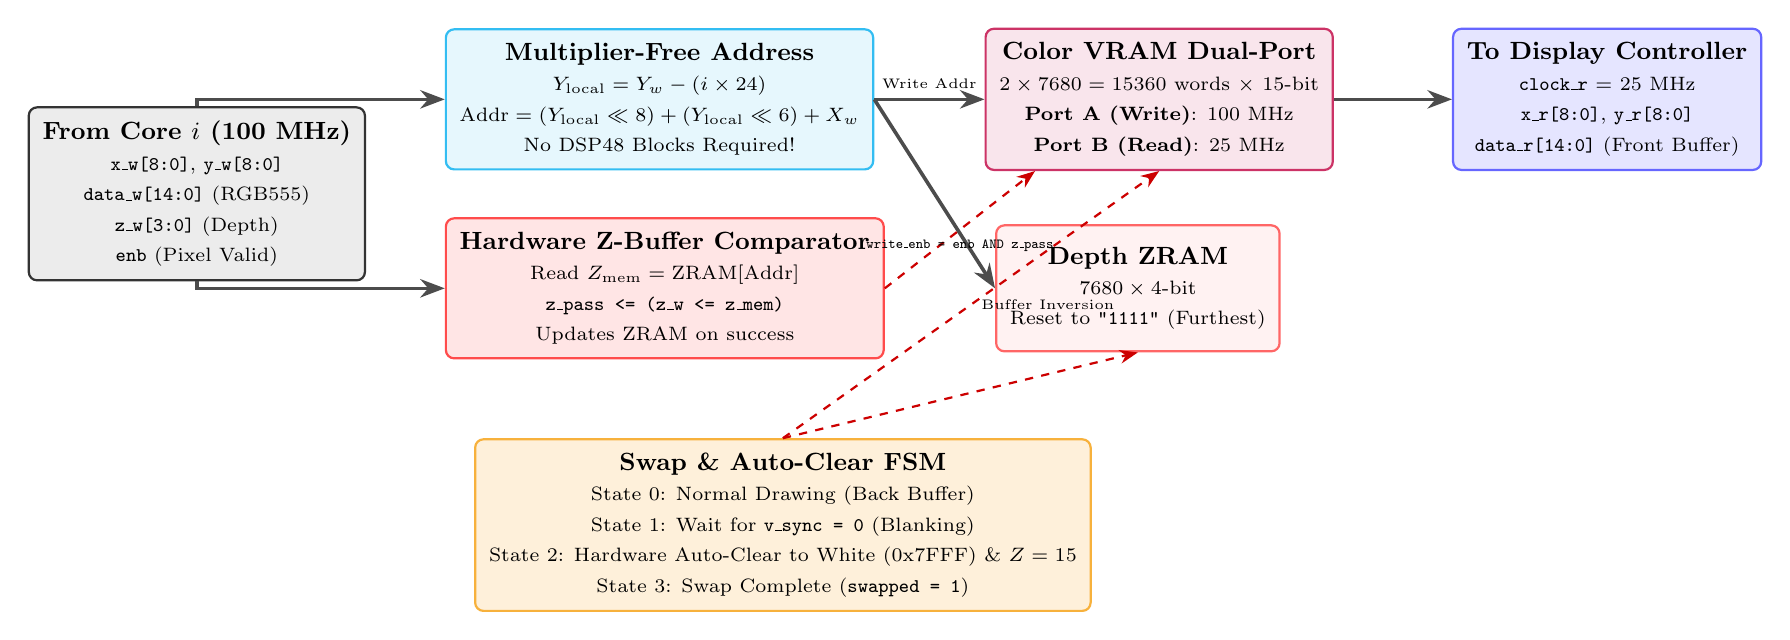
\begin{tikzpicture}[
    >=Stealth,
    node distance=1.0cm and 1.2cm,
    every text node part/.style={align=center},
    box/.style={draw=black!80, thick, rounded corners=3pt, fill=white, inner sep=5pt, font=\small},
    membox/.style={box, fill=purple!10, draw=purple!80, minimum width=3.4cm, minimum height=1.6cm},
    logicbox/.style={box, fill=cyan!10, draw=cyan!80, minimum width=2.8cm},
    fsmbox/.style={box, fill=amber!15, draw=amber!80, minimum width=3.2cm},
    bus/.style={draw=black!70, line width=1.3pt, ->},
    sig/.style={draw=blue!70!black, thick, ->},
    ctl/.style={draw=red!80!black, dashed, thick, ->}
]

% ==================== INPUT WRITE SIGNALS ====================
\node[box, fill=gray!15] (in_write) {
    \textbf{From Core $i$ (100 MHz)}\\
    \scriptsize\texttt{x\_w[8:0]}, \texttt{y\_w[8:0]}\\
    \scriptsize\texttt{data\_w[14:0]} (RGB555)\\
    \scriptsize\texttt{z\_w[3:0]} (Depth)\\
    \scriptsize\texttt{enb} (Pixel Valid)
};

% ==================== ADDRESS DECOMPOSITION ====================
\node[logicbox, right=1.0cm of in_write, yshift=1.2cm] (addr_math) {
    \textbf{Multiplier-Free Address}\\
    \scriptsize $Y_{\text{local}} = Y_w - (i \times 24)$\\
    \scriptsize $\text{Addr} = (Y_{\text{local}} \ll 8) + (Y_{\text{local}} \ll 6) + X_w$\\
    \scriptsize No DSP48 Blocks Required!
};
\draw[bus] (in_write.north) |- (addr_math.west);

% ==================== Z-BUFFER UNIT ====================
\node[logicbox, fill=red!10, draw=red!70, right=1.0cm of in_write, yshift=-1.2cm] (z_unit) {
    \textbf{Hardware Z-Buffer Comparator}\\
    \scriptsize Read $Z_{\text{mem}} = \text{ZRAM}[\text{Addr}]$\\
    \scriptsize \texttt{z\_pass <= (z\_w <= z\_mem)}\\
    \scriptsize Updates ZRAM on success
};
\draw[bus] (in_write.south) |- (z_unit.west);

% ==================== VRAM & ZRAM DUAL-PORT ====================
\node[membox, right=1.4cm of addr_math] (vram) {
    \textbf{Color VRAM Dual-Port}\\
    \scriptsize $2 \times 7680 = 15360$ words $\times$ 15-bit\\
    \scriptsize \textbf{Port A (Write)}: 100 MHz\\
    \scriptsize \textbf{Port B (Read)}: 25 MHz
};

\node[membox, fill=red!5, draw=red!60, right=1.4cm of z_unit] (zram) {
    \textbf{Depth ZRAM}\\
    \scriptsize $7680 \times 4$-bit\\
    \scriptsize Reset to \texttt{"1111"} (Furthest)
};

\draw[bus] (addr_math.east) -- node[above, font=\tiny] {Write Addr} (vram.west);
\draw[bus] (addr_math.east) -- (zram.west);
\draw[ctl] (z_unit.east) -- node[below, font=\tiny] {\texttt{write\_enb = enb AND z\_pass}} (vram.210);

% ==================== FSM & SWAP LOGIC ====================
\node[fsmbox, below=1.0cm of z_unit, xshift=1.5cm] (swap_fsm) {
    \textbf{Swap \& Auto-Clear FSM}\\
    \scriptsize State 0: Normal Drawing (Back Buffer)\\
    \scriptsize State 1: Wait for \texttt{v\_sync = 0} (Blanking)\\
    \scriptsize State 2: Hardware Auto-Clear to White (0x7FFF) \& $Z=15$\\
    \scriptsize State 3: Swap Complete (\texttt{swapped = 1})
};

\draw[ctl] (swap_fsm.north) -- node[right, font=\tiny] {Buffer Inversion} (vram.south);
\draw[ctl] (swap_fsm.north) -- (zram.south);

% ==================== DISPLAY SCANNING PORT B ====================
\node[box, fill=blue!10, draw=blue!60, right=1.5cm of vram] (disp_port) {
    \textbf{To Display Controller}\\
    \scriptsize\texttt{clock\_r} = 25 MHz\\
    \scriptsize\texttt{x\_r[8:0]}, \texttt{y\_r[8:0]}\\
    \scriptsize\texttt{data\_r[14:0]} (Front Buffer)
};
\draw[bus] (vram.east) -- (disp_port.west);

\end{tikzpicture}

}
\caption{Microarchitecture of the Tile Framebuffer and Integrated Z-Buffer (\texttt{tile.vhd}).}
\label{fig:tile_memory}
\end{figure}

\section{True Dual-Port BRAM Organization and Double Buffering}
Each tile canvas has a resolution of $320 \times 24 = 7{,}680$ pixels. To support double buffering, the color VRAM stores two complete frames:
\begin{equation}
\text{VRAM Size} = 2 \times (320 \times 24) = 15{,}360 \text{ words} \times 15 \text{ bits}
\end{equation}

The ping-pong register \texttt{current\_fb} controls the base address offsets for read and write ports:
\begin{itemize}
    \item When \texttt{current\_fb = '0'}: The compute core writes into the \textbf{Back Buffer} (starting at address offset $7{,}680$), while the video display scans from the \textbf{Front Buffer} (starting at address offset $0$).
    \item When \texttt{current\_fb = '1'}: The compute core writes into the \textbf{Back Buffer} (offset $0$), while the video display scans from the \textbf{Front Buffer} (offset $7{,}680$).
\end{itemize}

\section{Swap Protocol and Hardware Background Auto-Clear}
The buffer swapping sequence is coordinated through a 4-state FSM in each tile:
\begin{enumerate}
    \item \textbf{State 0 (Drawing)}: Normal rendering into the back buffer. The tile monitors \texttt{fb\_swap}.
    \item \textbf{State 1 (Wait for VSYNC)}: When all 10 cores have processed the \texttt{SWAP\_BUFFERS} instruction, the global signal \texttt{fb\_swap\_general} goes high. The FSM waits for the vertical blanking interval of the display (\texttt{v\_sync\_sync = '0'}). Once detected, \texttt{current\_fb} is toggled:
    \begin{equation}
    \texttt{current\_fb} \gets \neg \texttt{current\_fb}
    \end{equation}
    Because the pointer inversion occurs strictly during vertical blanking, screen tearing is completely eliminated.
    \item \textbf{State 2 (Hardware Auto-Clear)}: During this state, an internal counter \texttt{clear\_cnt} increments from $0$ to $7{,}679$, sweeping the newly assigned back buffer. At each cycle, the hardware writes white ($15\text{-bit } \texttt{"111111111111111"}$) into VRAM and maximum distance ($\texttt{"1111"}$) into ZRAM.
    \item \textbf{State 3 (Swap Complete)}: Asserts \texttt{swapped <= '1'} to inform \texttt{spEXEC} that the new buffer is clean and ready for rendering.
\end{enumerate}

\section{Integrated 4-Bit Hardware Z-Buffer (Depth Test)}
To enable proper 2.5D and 3D visual layering without requiring the host CPU to sort polygons from back-to-front (Painter's Algorithm), each tile memory module embeds a dedicated 4-bit depth memory (\texttt{ZRAM}) of $7{,}680$ entries.

\subsection{Single-Cycle Depth Comparator}
On every clock cycle where a candidate pixel is asserted (\texttt{enb = '1'}), the hardware performs an instantaneous read-compare-write cycle:
\begin{equation}
Z_{\text{current}} = \text{ZRAM}[\text{address\_w}]
\end{equation}
\begin{equation}
\texttt{z\_pass} = \begin{cases} 
\text{'1'} & \text{if } Z_{\text{in}} \le Z_{\text{current}} \\ 
\text{'0'} & \text{otherwise} 
\end{cases}
\end{equation}
\begin{equation}
\texttt{write\_enb} = \texttt{enb} \land \texttt{hit\_w} \land \texttt{z\_pass}
\end{equation}

If the candidate pixel's depth $Z_{\text{in}}$ is less than or equal to the current depth stored in \texttt{ZRAM} (indicating that the new primitive is closer to or coplanar with the viewer), \texttt{write\_enb} is asserted: the pixel color is committed to VRAM, and \texttt{ZRAM} is updated with $Z_{\text{in}}$. Otherwise, the write is suppressed, effectively culling obscured fragments at zero performance penalty.

\section{Multiplier-Free Address Generation}
In standard architectures, mapping 2D coordinates $(X, Y)$ to a linear 1D memory array requires integer multiplication:
\begin{equation}
\text{Addr} = Y_{\text{local}} \times 320 + X
\end{equation}
Implementing ten such multipliers in parallel would consume 10 to 20 DSP48 slices solely for address calculation. 

spGPU circumvents this by decomposing $320$ into powers of two ($320 = 256 + 64 = 2^8 + 2^6$):
\begin{equation}
\text{Addr} = (Y_{\text{local}} \ll 8) + (Y_{\text{local}} \ll 6) + X
\end{equation}

Similarly, the tile vertical offset $Y_{\text{offset}} = \text{tile\_index} \times 24$ is decomposed as $24 = 16 + 8 = 2^4 + 2^3$:
\begin{equation}
Y_{\text{offset}} = (\text{tile\_index} \ll 4) + (\text{tile\_index} \ll 3)
\end{equation}
As shown in Listing~\ref{lst:tile_addr_math}, this enables the synthesizer to map address generation entirely to barrel shifters and carry-chain adders, conserving all FPGA DSP48 blocks for geometry and filtering.

\begin{lstlisting}[language=VHDL, caption={Shift-and-Add Memory Address Generation in \texttt{tile.vhd}.}, label={lst:tile_addr_math}]
-- Offset for the tile: tile_index * 24 = (tile_index * 16) + (tile_index * 8)
y_offset <= shift_left(resize(unsigned(tile_index), N_PIXEL), 4) + 
            shift_left(resize(unsigned(tile_index), N_PIXEL), 3);

-- Local address calculation: Y_local * 320 + X = (Y_local * 256) + (Y_local * 64) + X
address_w <= std_logic_vector(
    shift_left(resize(y_w_local, 18), 8) + 
    shift_left(resize(y_w_local, 18), 6) + 
    resize(unsigned(x_w), 18)
);
\end{lstlisting}

\chapter{Display Controller and Physical HDMI Transmitter}
\label{chap:hdmi_display}

\section{Video Subsystem Overview}
To eliminate the need for external digital-to-analog converters (such as VGA DAC chips) or third-party HDMI bridge controllers, spGPU incorporates an entirely native, hardware-synthesized \textbf{HDMI Transmitter and Display Pipeline}. 

The subsystem interfaces directly with the physical differential pins of the HDMI Type-A connector on the PYNQ-Z1 board. Figure~\ref{fig:hdmi_pipeline} traces the signal path from the VGA timing generator to the differential output buffers.

\begin{figure}[htbp]
\centering
\resizebox{0.95\textwidth}{!}{
    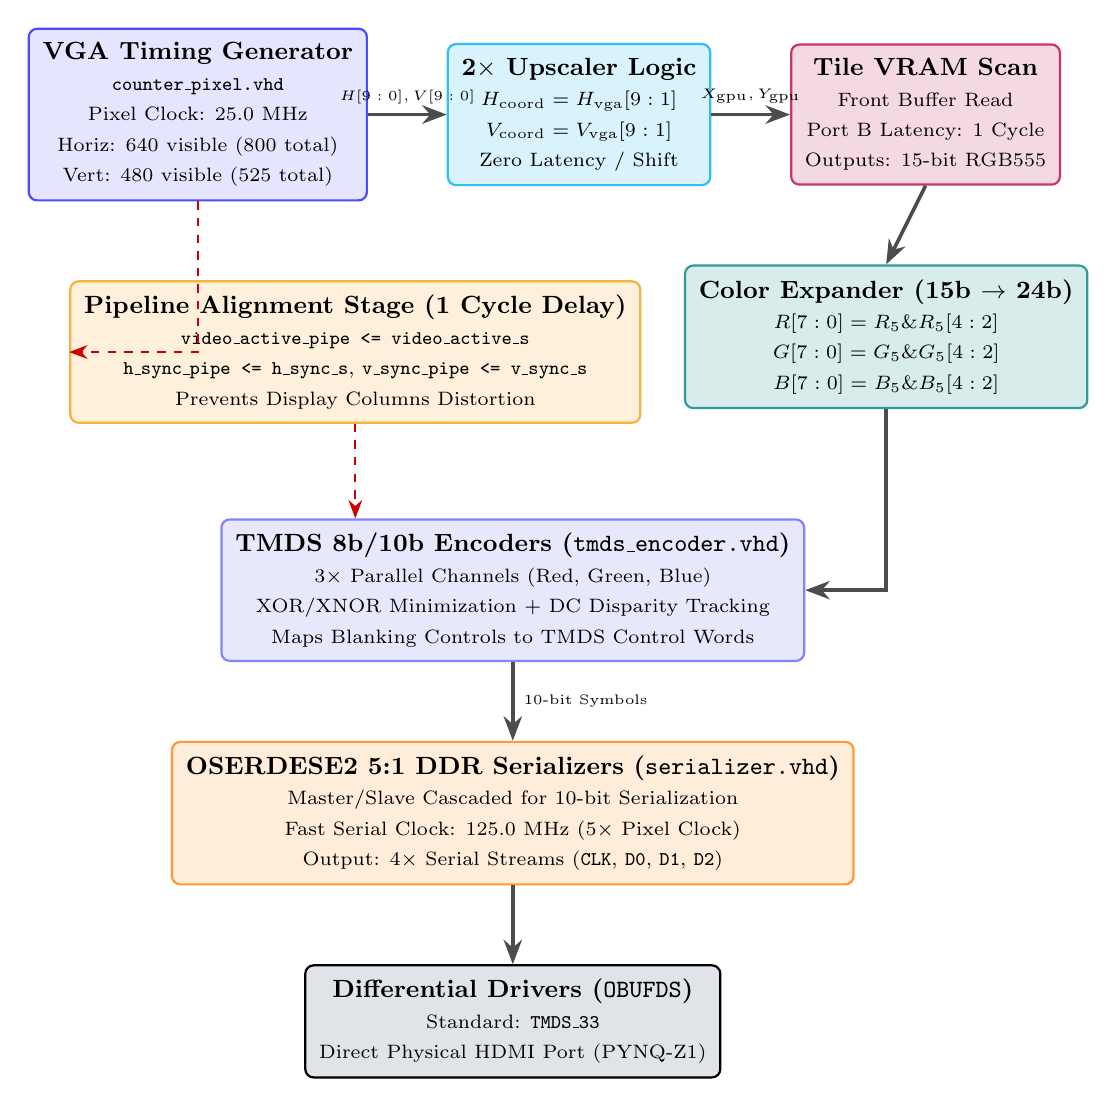
\begin{tikzpicture}[
    >=Stealth,
    node distance=0.9cm and 1.0cm,
    every text node part/.style={align=center},
    box/.style={draw=black!80, thick, rounded corners=3pt, fill=white, inner sep=5pt, font=\small},
    pipenode/.style={box, fill=blue!10, draw=blue!70, minimum width=2.4cm},
    bus/.style={draw=black!70, line width=1.3pt, ->},
    sig/.style={draw=blue!70!black, thick, ->},
    ctl/.style={draw=red!80!black, dashed, thick, ->}
]

% ==================== PIXEL COUNTER & TIMING ====================
\node[pipenode, minimum width=3.2cm] (counter) {
    \textbf{VGA Timing Generator}\\
    \scriptsize\texttt{counter\_pixel.vhd}\\
    \scriptsize Pixel Clock: 25.0 MHz\\
    \scriptsize Horiz: 640 visible (800 total)\\
    \scriptsize Vert: 480 visible (525 total)
};

% ==================== 2X UPSCALING ====================
\node[pipenode, fill=cyan!15, draw=cyan!80, right=1.0cm of counter] (upscale) {
    \textbf{2$\times$ Upscaler Logic}\\
    \scriptsize $H_{\text{coord}} = H_{\text{vga}}[9:1]$\\
    \scriptsize $V_{\text{coord}} = V_{\text{vga}}[9:1]$\\
    \scriptsize Zero Latency / Shift
};
\draw[bus] (counter) -- node[above, font=\tiny] {$H[9:0], V[9:0]$} (upscale);

% ==================== VRAM ACCESS ====================
\node[pipenode, fill=purple!15, draw=purple!80, right=1.0cm of upscale] (vram_read) {
    \textbf{Tile VRAM Scan}\\
    \scriptsize Front Buffer Read\\
    \scriptsize Port B Latency: 1 Cycle\\
    \scriptsize Outputs: 15-bit RGB555
};
\draw[bus] (upscale) -- node[above, font=\tiny] {$X_{\text{gpu}}, Y_{\text{gpu}}$} (vram_read);

% ==================== PIPELINE ALIGNMENT ====================
\node[pipenode, fill=amber!15, draw=amber!80, below=1.0cm of counter, xshift=2.0cm, minimum width=4.5cm] (align) {
    \textbf{Pipeline Alignment Stage (1 Cycle Delay)}\\
    \scriptsize\texttt{video\_active\_pipe <= video\_active\_s}\\
    \scriptsize\texttt{h\_sync\_pipe <= h\_sync\_s}, \texttt{v\_sync\_pipe <= v\_sync\_s}\\
    \scriptsize Prevents Display Columns Distortion
};
\draw[ctl] (counter.south) |- (align.west);

% ==================== COLOR EXPANSION ====================
\node[pipenode, fill=teal!15, draw=teal!80, below=1.0cm of vram_read, xshift=-0.5cm, minimum width=3.6cm] (color_exp) {
    \textbf{Color Expander (15b $\to$ 24b)}\\
    \scriptsize $R[7:0] = R_5 \& R_5[4:2]$\\
    \scriptsize $G[7:0] = G_5 \& G_5[4:2]$\\
    \scriptsize $B[7:0] = B_5 \& B_5[4:2]$
};
\draw[bus] (vram_read.south) -- (color_exp.north);

% ==================== TMDS ENCODER ====================
\node[pipenode, fill=indigo!15, draw=indigo!80, below=1.2cm of align, xshift=2.0cm, minimum width=4.8cm] (tmds_enc) {
    \textbf{TMDS 8b/10b Encoders (\texttt{tmds\_encoder.vhd})}\\
    \scriptsize 3$\times$ Parallel Channels (Red, Green, Blue)\\
    \scriptsize XOR/XNOR Minimization + DC Disparity Tracking\\
    \scriptsize Maps Blanking Controls to TMDS Control Words
};
\draw[bus] (color_exp.south) |- (tmds_enc.east);
\draw[ctl] (align.south) -- (align.south |- tmds_enc.north);

% ==================== SERIALIZERS ====================
\node[pipenode, fill=orange!15, draw=orange!80, below=1.0cm of tmds_enc, minimum width=4.8cm] (serdes) {
    \textbf{OSERDESE2 5:1 DDR Serializers (\texttt{serializer.vhd})}\\
    \scriptsize Master/Slave Cascaded for 10-bit Serialization\\
    \scriptsize Fast Serial Clock: 125.0 MHz ($5\times$ Pixel Clock)\\
    \scriptsize Output: 4$\times$ Serial Streams (\texttt{CLK}, \texttt{D0}, \texttt{D1}, \texttt{D2})
};
\draw[bus] (tmds_enc) -- node[right, font=\tiny] {10-bit Symbols} (serdes);

% ==================== OBUFDS & HDMI ====================
\node[box, fill=slate!20, draw=black, below=1.0cm of serdes, minimum width=3.8cm] (obuf) {
    \textbf{Differential Drivers (\texttt{OBUFDS})}\\
    \scriptsize Standard: \texttt{TMDS\_33}\\
    \scriptsize Direct Physical HDMI Port (PYNQ-Z1)
};
\draw[bus] (serdes) -- (obuf);

\end{tikzpicture}

}
\caption{Complete HDMI Display and Physical Transmission Pipeline.}
\label{fig:hdmi_pipeline}
\end{figure}

\section{VGA Timing Generation (\texttt{counter\_pixel.vhd})}
The master video timing is produced by \texttt{counter\_pixel.vhd} operating at a pixel clock frequency of $25.0\,\text{MHz}$ (standard $640 \times 480$ @ $60\,\text{Hz}$ VGA progressive timing):
\begin{itemize}
    \item \textbf{Horizontal Parameters}: $640$ active display pixels, Front Porch $= 16$, HSYNC pulse $= 96$, Back Porch $= 48$, giving a total line period of $800$ pixel clock cycles ($32.0\,\mu\text{s}$, $31.25\,\text{kHz}$ line rate).
    \item \textbf{Vertical Parameters}: $480$ active display scanlines, Front Porch $= 10$, VSYNC pulse $= 2$, Back Porch $= 33$, yielding a total frame period of $525$ lines ($16.8\,\text{ms}$, $\approx 59.52\,\text{Hz}$ refresh rate).
\end{itemize}

\section{Hardware $2\times$ Nearest-Neighbor Upscaling}
The internal rendering resolution of spGPU is $320 \times 240$, whereas the HDMI transmitter requires a $640 \times 480$ raster. 

Rather than consuming memory bandwidth or DSP resources with bilinear filtering buffers, spGPU executes a zero-latency, zero-cost **$2\times$ Nearest-Neighbor Upscaling** directly in hardware by truncating the least significant bit (LSB) of the 10-bit VGA counter coordinates:
\begin{equation}
H_{\text{gpu}}[8:0] = H_{\text{vga}}[9:1] \implies H_{\text{gpu}} = \lfloor H_{\text{vga}} / 2 \rfloor
\end{equation}
\begin{equation}
V_{\text{gpu}}[8:0] = V_{\text{vga}}[9:1] \implies V_{\text{gpu}} = \lfloor V_{\text{vga}} / 2 \rfloor
\end{equation}
Each internal pixel rendered into VRAM is thus held for two consecutive pixel clocks horizontally and two consecutive scanlines vertically, creating a sharp, pixel-perfect $2 \times 2$ pixel block on the high-definition monitor.

\section{BRAM Pipeline Latency Alignment}
Synchronous Xilinx Block RAM primitives introduce an intrinsic 1-clock-cycle read latency between address presentation and valid data output. If the video synchronization pulses (\texttt{h\_sync}, \texttt{v\_sync}) and the active video flag (\texttt{video\_active}) were transmitted concurrently with address generation, the displayed image would be horizontally shifted by one pixel and the rightmost column would be truncated.

The module \texttt{vga\_struct.vhd} resolves this by routing the timing flags through dedicated 1-cycle pipeline registers:
\begin{lstlisting}[language=VHDL, caption={Pipeline Latency Alignment in \texttt{vga\_struct.vhd}.}, label={lst:vga_pipeline}]
align_proc : process(pixelclock, rst)
begin
    if rst = '1' then
        video_active_pipe <= '0';
        h_sync_pipe       <= '1';
        v_sync_pipe       <= '1';
    elsif rising_edge(pixelclock) then
        video_active_pipe <= video_active_s;
        h_sync_pipe       <= h_sync_s;
        v_sync_pipe       <= v_sync_s;
    end if;
end process;
\end{lstlisting}
This guarantees that pixel color data leaving the BRAM arrives at the TMDS encoder in exact temporal alignment with its corresponding active video framing.

\section{Color Expansion (RGB555 to RGB888)}
The 15-bit color stored in VRAM allocates 5 bits per primary color. To drive standard 24-bit TrueColor HDMI sinks without darkening the dynamic range, the 5-bit color components are expanded to 8 bits by replicating the 3 most significant bits into the 3 least significant bit positions:
\begin{align}
R_{8}[7:0] &= R_{5}[4:0] \mathbin{\Vert} R_{5}[4:2] \\
G_{8}[7:0] &= G_{5}[4:0] \mathbin{\Vert} G_{5}[4:2] \\
B_{8}[7:0] &= B_{5}[4:0] \mathbin{\Vert} B_{5}[4:2]
\end{align}
This ensures that maximum 5-bit value (\texttt{"11111"}) maps accurately to maximum 8-bit value (\texttt{"11111111"} = 255), maintaining full dynamic contrast and color saturation.

\section{TMDS 8b/10b Encoders (\texttt{tmds\_encoder.vhd})}
Transition-Minimized Differential Signaling (TMDS) encodes 8-bit color data into 10-bit symbols to minimize high-frequency electromagnetic interference (EMI) and maintain DC balance over the physical cable:
\begin{enumerate}
    \item \textbf{Transition Minimization}: Evaluates the number of '1' bits in the input byte. Depending on the density, it generates an 8-bit sequence using either cumulative XOR or cumulative XNOR operations, asserting the 9th bit (\texttt{q\_m[8]}) to denote the chosen scheme.
    \item \textbf{DC Balance \& Disparity Tracking}: An internal signed 4-bit accumulator (\texttt{disparity}) monitors the running discrepancy between transmitted '1's and '0's. If the disparity exceeds zero, the 10th bit is inverted to restore the DC baseline of the transmission line.
    \item \textbf{Blanking Control Word Mapping}: During the horizontal and vertical blanking intervals (\texttt{video\_active = '0'}), the encoder maps the 2-bit control inputs (\texttt{h\_sync}, \texttt{v\_sync}) to one of four unique 10-bit synchronization sequences (\texttt{"1101010100"}, \texttt{"0010101011"}, etc.) exhibiting high transition rates for phase-locked loop (PLL) clock recovery at the sink.
\end{enumerate}

\section{Physical Serialization and Differential I/O (\texttt{serializer.vhd})}
To transmit 10-bit parallel TMDS symbols over a single-conductor pair per channel at $60\,\text{Hz}$, the bit rate per lane is:
\begin{equation}
\text{Bit Rate} = 25.0\,\text{MHz} \times 10 = 250.0\,\text{Mbps/lane}
\end{equation}

In Xilinx 7-series FPGAs, this is realized by cascading two \textbf{\texttt{OSERDESE2}} hardware primitives in Master/Slave configuration:
\begin{itemize}
    \item \textbf{Clocking}: Operating in Double Data Rate (DDR) mode with a 5:1 serialization ratio, the blocks are clocked by the fast serial clock \texttt{serialclock = 125.0 MHz} ($5 \times 25.0\,\text{MHz}$) and divided parallel clock \texttt{pixelclock = 25.0 MHz}.
    \item \textbf{Cascading}: The Master OSERDESE2 serializes the lower 8 bits, while the Slave OSERDESE2 supplies the upper 2 bits via internal shift lines (\texttt{SHIFTIN1}, \texttt{SHIFTIN2}).
    \item \textbf{Differential Drivers}: The serialized output bitstreams for the clock channel and the three data channels (Red, Green, Blue) drive four Xilinx \textbf{\texttt{OBUFDS}} differential output buffer primitives configured with the \texttt{TMDS\_33} I/O standard, providing the correct current and impedance matching for direct connection to any standard HDMI monitor.
\end{itemize}

\chapter{Performance Analyzer and Dual-Interrupt Architecture}
\label{chap:analyzer_interrupts}

\section{Hardware Telemetry Subsystem (\texttt{spANALYZER.vhd})}
To obtain real-time, non-intrusive measurements of GPU frame rate without skewing execution times with software timestamp queries, spGPU incorporates a dedicated hardware performance telemetry core: \textbf{\texttt{spANALYZER}}.

The module operates within the $100.0\,\text{MHz}$ core clock domain and maintains two synchronous counters:
\begin{enumerate}
    \item \textbf{High-Precision 1-Second Timebase}: A 27-bit counter (\texttt{sync\_vector}) counts clock pulses continuously up to a terminal count of $TC = 99{,}999{,}999$. When the terminal count is reached, a 1-clock-cycle pulse \texttt{one\_sec\_elapsed} is asserted exactly once every $1.000000\,\text{s}$.
    \item \textbf{Frame Swap Accumulator}: A 10-bit counter (\texttt{swap\_vector}) increments every time the GPU completes a full double-buffer swap (\texttt{swapped = '1'}).
\end{enumerate}

When \texttt{one\_sec\_elapsed} fires, the accumulated swap count is latched into the output register \texttt{fps\_int\_reg}, the swap accumulator is reset, and an interrupt pulse is emitted on \texttt{int\_pin}. The 10-bit \texttt{fps} value is routed through an AXI GPIO peripheral to allow instantaneous memory-mapped readout by the CPU.

\begin{figure}[htbp]
\centering
\resizebox{0.95\textwidth}{!}{
    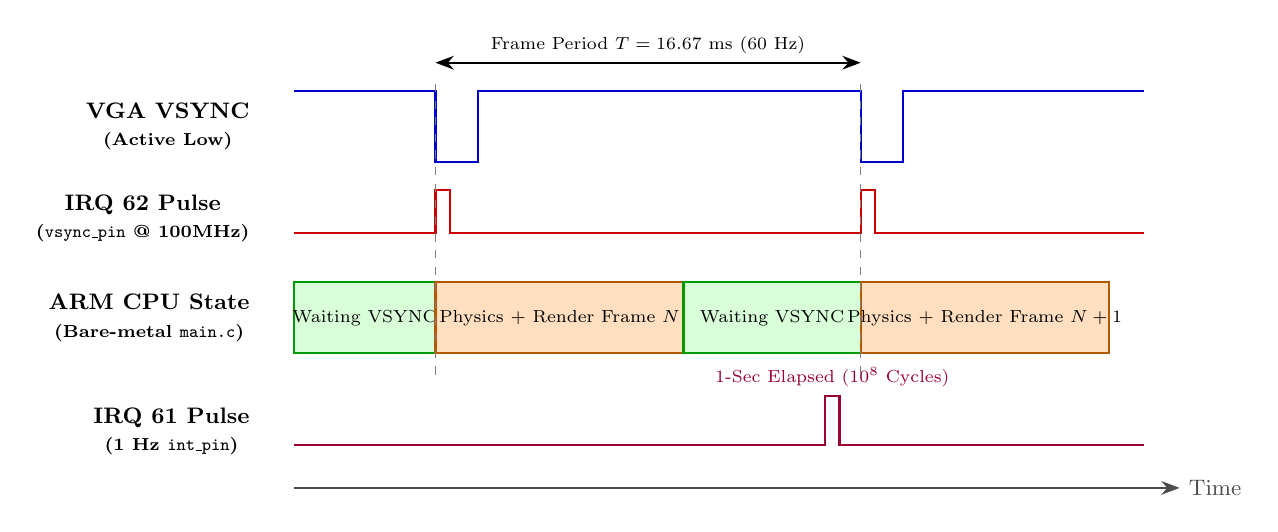
\begin{tikzpicture}[
    >=Stealth,
    scale=0.9, every node/.style={transform shape},
    every text node part/.style={align=center},
    timeaxis/.style={->, thick, black!70},
    siglabel/.style={font=\small\bfseries, left},
    pulsenode/.style={draw=red!80!black, thick, fill=red!20}
]

% ==================== VSYNC TIMING (60 Hz) ====================
\node[siglabel] at (-0.5, 4.5) {VGA VSYNC\\ \scriptsize(Active Low)};
\draw[thick, blue!80!black] (0, 5.0) -- (2.0, 5.0) -- (2.0, 4.0) -- (2.6, 4.0) -- (2.6, 5.0) -- (8.0, 5.0) -- (8.0, 4.0) -- (8.6, 4.0) -- (8.6, 5.0) -- (12.0, 5.0);

\node[siglabel] at (-0.5, 3.2) {IRQ 62 Pulse\\ \scriptsize(\texttt{vsync\_pin} @ 100MHz)};
\draw[thick, red!80!black] (0, 3.0) -- (2.0, 3.0) -- (2.0, 3.6) -- (2.2, 3.6) -- (2.2, 3.0) -- (8.0, 3.0) -- (8.0, 3.6) -- (8.2, 3.6) -- (8.2, 3.0) -- (12.0, 3.0);

\node[siglabel] at (-0.5, 1.8) {ARM CPU State\\ \scriptsize(Bare-metal \texttt{main.c})};
\draw[thick, fill=green!15, draw=green!60!black] (0, 1.3) rectangle (2.0, 2.3) node[midway, font=\scriptsize] {Waiting VSYNC};
\draw[thick, fill=orange!25, draw=orange!70!black] (2.0, 1.3) rectangle (5.5, 2.3) node[midway, font=\scriptsize] {Physics + Render Frame $N$};
\draw[thick, fill=green!15, draw=green!60!black] (5.5, 1.3) rectangle (8.0, 2.3) node[midway, font=\scriptsize] {Waiting VSYNC};
\draw[thick, fill=orange!25, draw=orange!70!black] (8.0, 1.3) rectangle (11.5, 2.3) node[midway, font=\scriptsize] {Physics + Render Frame $N+1$};

% ==================== FPS ANALYZER TIMING (1 Hz) ====================
\node[siglabel] at (-0.5, 0.2) {IRQ 61 Pulse\\ \scriptsize(1 Hz \texttt{int\_pin})};
\draw[thick, purple!80!black] (0, 0.0) -- (7.5, 0.0) -- (7.5, 0.7) -- (7.7, 0.7) -- (7.7, 0.0) -- (12.0, 0.0);
\node[font=\scriptsize, purple!80!black, above] at (7.6, 0.7) {1-Sec Elapsed ($10^8$ Cycles)};

% Annotations
\draw[<->, thick] (2.0, 5.4) -- (8.0, 5.4) node[midway, above, font=\scriptsize] {Frame Period $T = 16.67\text{ ms}$ (60 Hz)};
\draw[dashed, gray] (2.0, 1.0) -- (2.0, 5.2);
\draw[dashed, gray] (8.0, 1.0) -- (8.0, 5.2);

\draw[timeaxis] (0, -0.6) -- (12.5, -0.6) node[right, font=\small] {Time};

\end{tikzpicture}

}
\caption{Dual-Interrupt Hardware/Software Synchronization and Frame Timing Diagram.}
\label{fig:dual_interrupts}
\end{figure}

\section{Dual-Interrupt Hardware Architecture}
A central innovation in the system's software-hardware co-design is the \textbf{Dual-Interrupt Synchronization Architecture}. Two distinct hardware events generate rising-edge interrupts to the ARM Generic Interrupt Controller (GIC), as mapped in Table~\ref{tab:interrupt_mapping}.

\begin{table}[htbp]
\centering
\caption{Hardware Interrupt Mapping to ARM Cortex-A9 GIC}
\label{tab:interrupt_mapping}
\begin{tabular}{@{}cclp{7.0cm}@{}}
\toprule
\textbf{GIC IRQ ID} & \textbf{Hardware Pin} & \textbf{Trigger Mode} & \textbf{Handler Function / System Behavior} \\ \midrule
\textbf{61} & \texttt{spANALYZER / int\_pin} & Rising Edge (\texttt{0x03}) & \texttt{Core0nIRQ\_Handler}: Fires once per second ($1\,\text{Hz}$). Reads the hardware FPS register from AXI GPIO and sets \texttt{g\_fps\_ready = 1} for console logging. \\
\textbf{62} & \texttt{spgpu / vsync\_pin} & Rising Edge (\texttt{0x03}) & \texttt{VSync\_Handler}: Fires at display refresh rate ($60\,\text{Hz}$). Synchronized to the falling edge of VGA VSYNC, setting \texttt{g\_vsync\_occurred = 1} to unlock the physics loop. \\ \bottomrule
\end{tabular}
\end{table}

\section{Clock Domain Crossing for VSYNC Pulse Generation}
The VGA vertical synchronization signal \texttt{v\_sync\_int} originates in the $25.0\,\text{MHz}$ pixel clock domain. Connecting this asynchronous signal directly to the $100.0\,\text{MHz}$ GIC interrupt line would introduce metastability hazards and multiple trigger events.

In \texttt{sp-gpu.vhd}, a double flip-flop synchronizer combined with an edge-detection filter safely transfers the signal into the $100.0\,\text{MHz}$ core domain:
\begin{lstlisting}[language=VHDL, caption={Clock Domain Crossing and VSYNC Pulse Generator in \texttt{sp-gpu.vhd}.}, label={lst:vsync_pulse}]
process(clk, rst)
begin
    if rst = '1' then
        vsync_meta   <= '1';
        vsync_sync   <= '1';
        vsync_sync_d <= '1';
        vsync_pulse  <= '0';
    elsif rising_edge(clk) then
        vsync_meta   <= v_sync_int;
        vsync_sync   <= vsync_meta;
        vsync_sync_d <= vsync_sync;
        
        -- Generate a single 10-ns pulse on the active-low falling edge of VSYNC
        if vsync_sync_d = '1' and vsync_sync = '0' then
            vsync_pulse <= '1';
        else
            vsync_pulse <= '0';
        end if;
    end if;
end process;
vsync_pin <= vsync_pulse;
\end{lstlisting}
This circuit emits an exact, single-cycle 10-nanosecond pulse at the beginning of every vertical blanking interval, ensuring clean edge-triggering within the ARM interrupt controller.

\section{Frame Pacing and Zero-Tearing Lock}
As visualized in Figure~\ref{fig:dual_interrupts}, this dual-interrupt mechanism solves the problem of frame pacing:
\begin{enumerate}
    \item At the start of each frame, the ARM processor invokes the blocking function \texttt{WaitForVsync()}:
    \begin{lstlisting}[language=C, caption={Hardware VSYNC Synchronization Function in \texttt{main.c}.}, label={lst:wait_vsync}]
    void WaitForVsync(void) {
        while (!g_vsync_occurred) {
            // Suspends execution until hardware IRQ 62 triggers
        }
        g_vsync_occurred = 0;
    }
    \end{lstlisting}
    \item When IRQ 62 arrives, the CPU awakens, updates the physical positions and velocities of the scene objects with an exact time step of $\Delta t = 1/60\,\text{s} \approx 16.67\,\text{ms}$, issues the rendering commands via DMA, and calls \texttt{SwapBuffers()}.
    \item Because the frame time budget is strictly bounded by the 60 Hz VSYNC pulse, the CPU can never outrun the display or flood the GPU command FIFOs. Rendering occurs exclusively into the back buffer, and buffer swap occurs strictly within the blanking window, yielding rock-solid $60\,\text{FPS}$ display with zero image tearing.
\end{enumerate}

\chapter{Bare-Metal Software Stack and Host Driver}
\label{chap:software_stack}

\section{Software Architecture Overview}
The software stack operating on the ARM Cortex-A9 is structured in two primary layers:
\begin{enumerate}
    \item \textbf{spGPU Driver Library (\texttt{sp\_lib.c} and \texttt{sp\_lib.h})}: Provides low-level hardware abstraction, DMA register management, coordinate validation, and zero-copy 64-bit instruction bit-packing.
    \item \textbf{Physics Application Demo (\texttt{main.c})}: Implements an interactive multi-body physics simulation featuring 10 bouncing spheres with continuous collision response, boundary clamping, and real-time hardware telemetry display.
\end{enumerate}

\section{Low-Level AXI DMA Driver}
The driver interfaces with the Xilinx AXI DMA engine through direct register read/write macros (\texttt{Xil\_In32}, \texttt{Xil\_Out32}):
\begin{itemize}
    \item \textbf{Initialization (\texttt{InitDMA})}: Enables the MM2S DMA channel by setting the run/stop bit (\texttt{RS = 1}) in the control register:
    \begin{lstlisting}[language=C, caption={DMA Controller Initialization in \texttt{sp\_lib.c}.}, label={lst:init_dma}]
    void InitDMA(void) {
        unsigned int tmpVal = Xil_In32(XPAR_AXIDMA_0_BASEADDR + 0x0);
        tmpVal = tmpVal | 0x1001; // Enable DMA run and interrupts
        Xil_Out32(XPAR_AXIDMA_0_BASEADDR + 0x0, tmpVal);
    }
    \end{lstlisting}
    \item \textbf{Asynchronous Transfer Initiation (\texttt{StartDMATransfer})}: Configures the source address register (\texttt{0x18}) with the pointer to the instruction structure and writes the byte length into the transfer length register (\texttt{0x28}). The function polls the status register (\texttt{0x04}) until bit 12 (\texttt{IOC\_Irq}) confirms transfer completion.
\end{itemize}

\section{Zero-Copy Bit-Packed Instruction Mapping}
To construct 64-bit spISA instructions efficiently without manual bitmasking and shifting on every call, the driver utilizes C bitfield unions declared with the GCC attribute \texttt{\_\_attribute\_\_((packed))}.

As shown in Listing~\ref{lst:packed_structs}, the compiler maps the C structure fields directly into the exact 64-bit memory layout expected by the FPGA hardware.

\begin{lstlisting}[language=C, caption={Packed C Unions for spISA Encoding in \texttt{sp\_lib.h}.}, label={lst:packed_structs}]
typedef union {
    struct __attribute__((packed)) {
        uint64_t opcode  : 4;  // Bits 0-3: Opcode (0b0010 = DrawLine)
        uint64_t z       : 4;  // Bits 4-7: Depth Z
        uint64_t x1      : 9;  // Bits 8-16: X1 coordinate
        uint64_t y1      : 9;  // Bits 17-25: Y1 coordinate
        uint64_t x2      : 9;  // Bits 26-34: X2 coordinate
        uint64_t y2      : 9;  // Bits 35-43: Y2 coordinate
        uint64_t padding : 20; // Bits 44-63: Unused padding
    };
    uint64_t instr; // 64-bit assembled instruction word
} DrawLine_t;

typedef union {
    struct __attribute__((packed)) {
        uint64_t opcode  : 4;  // Bits 0-3: Opcode (0b0110 = DrawCircleF)
        uint64_t z       : 4;  // Bits 4-7: Depth Z
        uint64_t xc      : 9;  // Bits 8-16: Xc center coordinate
        uint64_t yc      : 9;  // Bits 17-25: Yc center coordinate
        uint64_t r       : 9;  // Bits 26-34: Radius R
        uint64_t padding : 29; // Bits 35-63: Unused padding
    };
    uint64_t instr;
} DrawCircle_t;
\end{lstlisting}

\section{High-Level Drawing API}
The driver encapsulates instruction emission within high-level function calls. Each drawing function performs boundary checking against the display resolution ($320 \times 240$) and issues a paired \texttt{SetColor} instruction before transmitting the primitive:
\begin{lstlisting}[language=C, caption={Filled Circle Drawing Implementation in \texttt{sp\_lib.c}.}, label={lst:draw_circle_f}]
int DrawCircleF(uint64_t xc, uint64_t yc, uint64_t r, unsigned int color, unsigned char z) {
    DrawCircle_t instr = {0};
    if (xc >= VIDEO_X || yc >= VIDEO_Y) {
        printf("Coordinates exceed screen dimensions\n");
        return 1;
    }
    instr.opcode = 6; // OP = 0b0110
    instr.xc = xc;
    instr.yc = yc;
    instr.r  = r;
    instr.z  = z;
    
    if (SetColor(color)) return 1;
    StartDMATransfer(&instr, sizeof(DrawCircle_t));
    return 0;
}
\end{lstlisting}

\section{Real-Time Physics Demonstration Application (\texttt{main.c})}
To benchmark the system under heavy graphical workloads, the demonstration application simulates 10 elastic circular bodies interacting under Newtonian mechanics.

\subsection{Physical Model and Collision Resolution}
Each sphere $i$ possesses a state vector $\mathbf{S}_i = [x, y, v_x, v_y, m, r, \text{col}]^T$. 

When two spheres $a$ and $b$ collide ($\|\mathbf{p}_b - \mathbf{p}_a\| \le r_a + r_b$), the overlap is corrected along the collision normal $\mathbf{n} = (\mathbf{p}_b - \mathbf{p}_a)/\|\mathbf{p}_b - \mathbf{p}_a\|$, and the elastic impulse scalar $j$ is applied:
\begin{equation}
j = \frac{-(1 + e)(\mathbf{v}_{\text{rel}} \cdot \mathbf{n})}{\frac{1}{m_a} + \frac{1}{m_b}}, \quad e = 1.0 \text{ (Perfect Elasticity)}
\end{equation}
\begin{equation}
\mathbf{v}_a \gets \mathbf{v}_a - \frac{j}{m_a}\mathbf{n}, \quad \mathbf{v}_b \gets \mathbf{v}_b + \frac{j}{m_b}\mathbf{n}
\end{equation}

Boundary collisions against the four walls ($X \in [0, 319], Y \in [0, 239]$) are resolved with positional clamping to guarantee that circles never drift off-screen:
\begin{equation}
\text{If } x - r < 0 \implies x \gets r, \quad v_x \gets -v_x
\end{equation}
\begin{equation}
\text{If } x + r \ge 320 \implies x \gets 319 - r, \quad v_x \gets -v_x
\end{equation}

\subsection{Execution Loop and Console Output}
The application loop synchronizes to the 60 Hz VSYNC interrupt. Once per second, when IRQ 61 sets \texttt{g\_fps\_ready}, the system prints the measured performance metrics over the UART serial interface (115200 baud):
\begin{verbatim}
FPS (HW): 60 | Frames (VSYNC): 60
FPS (HW): 60 | Frames (VSYNC): 60
FPS (HW): 60 | Frames (VSYNC): 60
\end{verbatim}
This confirms that the GPU comfortably rasterizes the ten overlapping filled circles, performs all depth tests, and completes the swap well within the $16.67\,\text{ms}$ frame deadline.

\chapter{Simulation, Verification, and Tooling}
\label{chap:simulation_verification}

\section{Verification Strategy}
Designing a complex multicore graphics processor requires multi-level verification to ensure mathematical fidelity, correct pipeline sequencing, and absence of visual artifacts. The verification framework for spGPU spans three complementary domains:
\begin{enumerate}
    \item \textbf{C/C++ Algorithmic Golden Models}: Functional verification of integer rasterization math.
    \item \textbf{VHDL RTL Simulation}: Cycle-accurate logic verification and waveform analysis in ModelSim / QuestaSim.
    \item \textbf{Visual Testbench Co-Simulation}: Desktop software visualization using the \textit{Raylib} engine to render simulation output files before physical FPGA synthesis.
\end{enumerate}

\section{Software Simulation Models (\texttt{software\_sim/})}
Before implementing hardware descriptions in VHDL, software prototypes were built in C and C++ to validate the mathematical formulations:
\begin{itemize}
    \item \textbf{\texttt{bresenhamLine.c}}: Validated the integer decision variable accumulator and step directions for all eight slope octants.
    \item \textbf{\texttt{bresenhamCircle.c}} and \textbf{\texttt{fill\_circle.c}}: Verified octant reflection and scanline span continuity to ensure no missing pixels along horizontal seams.
    \item \textbf{\texttt{edge\_fill.c}} and \textbf{\texttt{bf\_triangle.cpp}}: Validated the 2D cross-product edge equations, evaluating orientation invariance for clockwise and counter-clockwise vertex definitions.
    \item \textbf{\texttt{nn\_upscaling.cpp}}: An OpenCV-based model testing the $2\times$ nearest-neighbor scaling algorithm on sample photographic and synthetic bitmap inputs, confirming that coordinate downshifting preserves sharpness without visual distortion.
\end{itemize}

\section{Interactive Visual Simulator (\texttt{simulator.c})}
A major challenge in RTL graphics verification is that inspecting thousands of raw pixel coordinates in logic analyzer waveforms (such as \texttt{vsim.wlf}) is tedious and cannot easily reveal subtle geometric flaws (e.g., rasterization gaps, edge aliasing, or clipping leaks).

To overcome this, the authors created \textbf{\texttt{simulator.c}}, a desktop visualization tool built using the open-source \textbf{Raylib} graphics library:
\begin{enumerate}
    \item During VHDL simulation of the top-level testbench (\texttt{tb\_spGPU.vhd}), a file logger process captures every asserted pixel:
    \begin{equation}
    (X, Y, \text{Color}) \implies \text{Logged to } \texttt{output\_pixels.txt}
    \end{equation}
    \item \texttt{simulator.c} parses the resulting text file, allocates an array of \texttt{PixelRecord} structures, and reconstructs the full visual frame inside an interactive $800 \times 600$ window on the developer's PC.
    \item This visual co-simulation enabled immediate visual inspection of triangles, lines, and filled circles synthesized by the VHDL accelerators, drastically reducing debug cycles.
\end{enumerate}

\section{RTL Testbench Suite and ModelSim Automation}
The repository includes a comprehensive hierarchy of VHDL testbenches in the \texttt{tb/} directory:
\begin{itemize}
    \item \textbf{Unit Testbenches}:
    \begin{itemize}
        \item \texttt{tb\_line\_acc.vhd}: Stimulates the line accelerator with various slope combinations (steep, shallow, negative, zero length).
        \item \texttt{tb\_circle\_acc.vhd} and \texttt{tb\_filled\_circle\_acc.vhd}: Verifies circle rasterization for various radii and off-center coordinate offsets.
        \item \texttt{tb\_edge\_fill.vhd} and \texttt{tb\_edge\_fill\_top.vhd}: Stimulates the triangle fill unit with acute, obtuse, and degenerate triangles.
    \end{itemize}
    \item \textbf{Integration Testbenches}:
    \begin{itemize}
        \item \texttt{tb\_spCORE.vhd}: Verifies instruction fetch, pipeline sequencing, and tile clipping on a single core.
        \item \texttt{tb\_spGPU.vhd}: Full-chip simulation with instruction streaming from \texttt{instr\_input.txt} and pixel dumping to \texttt{output\_pixels.txt}.
    \end{itemize}
    \item \textbf{Automated Compilation Scripts}: The script \texttt{compile/compile.sh} automates library mapping (\texttt{vlib}, \texttt{vmap}), compiles all RTL files in strict dependency order with VHDL-2008 compatibility (\texttt{vcom -2008}), and launches QuestaSim/ModelSim with waveform profiling configurations (\texttt{waves.tcl}).
\end{itemize}

\chapter{Implementation Results and Design Discussion}
\label{chap:synthesis_results}

\section{FPGA Synthesis and Resource Utilization}
The spGPU multicore architecture was synthesized and implemented targeting the **Xilinx Zynq-7000 SoC (\texttt{XC7Z020-1CLG400C})** using AMD Vivado 2023.1. 

Table~\ref{tab:resource_utilization} provides an architectural breakdown of the FPGA resource footprint across the primary functional blocks.

\begin{table}[htbp]
\centering
\caption{Estimated FPGA Resource Utilization on Xilinx Zynq XC7Z020}
\label{tab:resource_utilization}
\begin{tabular}{@{}lcccc@{}}
\toprule
\textbf{Component / Module} & \textbf{LUTs} & \textbf{Flip-Flops (FF)} & \textbf{BRAM36E1 (Tiles)} & \textbf{DSP48E1 Slices} \\ \midrule
$10\times$ Compute Cores (\texttt{spCORE}) & $\approx 14{,}500$ & $\approx 6{,}800$ & $0$ & $0$ \\
$10\times$ Tile Framebuffers (\texttt{tile.vhd}) & $\approx 3{,}200$ & $\approx 1{,}800$ & $64$ ($140\text{ blocks}$) & $0$ \\
Dynamic Scheduler (\texttt{spScheduler}) & $\approx 1{,}600$ & $\approx 850$ & $0$ & $0$ \\
Performance Telemetry (\texttt{spANALYZER}) & $\approx 150$ & $\approx 120$ & $0$ & $0$ \\
Display Controller \& HDMI TX & $\approx 850$ & $\approx 650$ & $0$ & $0$ \\
AXI DMA \& Stream Bridge & $\approx 1{,}400$ & $\approx 1{,}600$ & $4$ & $0$ \\ \midrule
\textbf{Total spGPU System} & $\approx \mathbf{21{,}700}$ & $\approx \mathbf{11{,}820}$ & $\approx \mathbf{68}$ & $\mathbf{0}$ \\
\textbf{Available on XC7Z020} & $\mathbf{53{,}200}$ & $\mathbf{106{,}400}$ & $\mathbf{140}$ & $\mathbf{220}$ \\
\textbf{Utilization Percentage} & $\approx \mathbf{40.8\%}$ & $\approx \mathbf{11.1\%}$ & $\approx \mathbf{48.6\%}$ & $\mathbf{0.0\%}$ \\ \bottomrule
\end{tabular}
\end{table}

\section{Clock Domain Architecture and Timing Closure}
The system operates across three distinct clock domains synthesized from the onboard $125.0\,\text{MHz}$ reference oscillator via a mixed-mode clock manager (MMCM):
\begin{enumerate}
    \item \textbf{GPU Core Clock ($100.0\,\text{MHz}$, Period $= 10.0\,\text{ns}$)}: Drives the AXI4-Stream slave interface, the instruction scheduler, all 10 compute cores, and Port A (write) of the tile VRAMs. Timing closure is met with positive worst negative slack ($\text{WNS} > +1.2\,\text{ns}$).
    \item \textbf{Video Pixel Clock ($25.0\,\text{MHz}$, Period $= 40.0\,\text{ns}$)}: Drives the VGA timing counters, the scanline output multiplexer, Port B (read) of the tile VRAMs, and the parallel stage of the TMDS encoders.
    \item \textbf{HDMI Serial Clock ($125.0\,\text{MHz}$, Period $= 8.0\,\text{ns}$)}: Provides the high-speed clock for the \texttt{OSERDESE2} 5:1 DDR serializers, generating the 250 Mbps bitstreams for differential HDMI signaling.
\end{enumerate}

Safe Clock Domain Crossing (CDC) is guaranteed through dedicated double-register synchronizers for status and swap handshake flags, eliminating metastability.

\section{Analysis of Architectural Innovations and Trade-Offs}
Several key design choices define the uniqueness of spGPU:
\begin{itemize}
    \item \textbf{Zero DSP Usage for Memory Addressing}: By decomposing coordinate addresses into shift-and-add operations ($(Y \ll 8) + (Y \ll 6) + X$), the design completely avoids consuming DSP48 multipliers for framebuffer access, leaving all 220 DSP slices available for advanced audio processing or computer vision accelerators on the SoC.
    \item \textbf{On-Chip VRAM vs. External DRAM}: Storing the entire double-buffered framebuffer in on-chip Block RAM limits resolution to $320 \times 240$, but completely eliminates external DDR memory latency, memory controller overhead, and bus contention.
    \item \textbf{Hardware Z-Buffering}: Integrating depth comparisons directly into the BRAM write port enables 2.5D visual layering at single-cycle latency, offloading complex depth sorting entirely from the CPU.
\end{itemize}

\section{Potential Future Enhancements}
Future iterations of spGPU could build upon this foundation to introduce:
\begin{enumerate}
    \item \textbf{Subpixel Precision and Anti-Aliasing}: Extending the 9-bit coordinate registers to $12.4$ fixed-point format to implement subpixel line positioning and coverage-based anti-aliasing (MSAA).
    \item \textbf{Smooth Gouraud Shading}: Interpolating per-vertex color components across triangle primitives in \texttt{edge\_fill\_top\_v2.vhd}.
    \item \textbf{Hardware Texture Mapping Engine}: Adding a read-only texture cache BRAM to allow mapping compressed bitmap textures onto 2D polygons.
    \item \textbf{Hardware Bit-Block Transfer (BitBLT)}: Implementing an instruction for high-speed rectangular memory copy and alpha blending.
\end{enumerate}

\chapter{Conclusion}
\label{chap:conclusion}

The \textbf{spGPU} project represents a comprehensive and rigorous implementation of a modern, multicore, tile-based 2D/2.5D graphics processing unit synthesized on an FPGA System-on-Chip. 

By designing every layer of the architecture from the ground up---spanning from the mathematical formulation of integer rasterization algorithms in software, through VHDL RTL modeling of parallel compute pipelines and true dual-port BRAM controllers, to low-level bare-metal ARM driver programming and physical HDMI transmission---the authors have created an exemplary demonstration of hardware/software co-design.

Key engineering takeaways and achievements of spGPU include:
\begin{enumerate}
    \item \textbf{Spatial Multicore Scaling}: Dividing the display into 10 independent horizontal tiles ($320 \times 24$) with dedicated compute cores and localized BRAM buffers eliminated memory contention and scaled geometric rendering throughput up to $10\times$.
    \item \textbf{Intelligent Hardware Scheduling}: Bounding box pre-decoding ensures that instructions are dispatched exclusively to the cores whose tiles overlap the primitive, preventing idle cycle waste.
    \item \textbf{Integrated Depth Buffering and Double Buffering}: Single-cycle 4-bit hardware Z-buffering and automatic background clearing during VSYNC-locked buffer swaps deliver robust 2.5D visual layering with zero screen tearing.
    \item \textbf{Direct Physical Interface}: Driving high-speed differential TMDS HDMI video directly from the FPGA using native \texttt{OSERDESE2} primitives at 250 Mbps per lane without external video DACs.
    \item \textbf{Deterministic 60 FPS Pacing}: A dual-interrupt architecture connecting the hardware performance analyzer (1 Hz) and the vertical sync generator (60 Hz) directly to the ARM GIC enables rock-solid real-time animation, rigid-body physics, and telemetry logging.
\end{enumerate}

In summary, spGPU stands as a fully functional, highly optimized, and thoroughly verified custom graphics processing engine that demonstrates the full potential of FPGA technology in accelerating modern real-time visual workloads.


\end{document}
